\documentclass[11pt,a4paper]{article}

\usepackage[utf8]{inputenc}
\usepackage[T1]{fontenc}
\usepackage[english]{babel}
\usepackage{lmodern}
\usepackage{amsmath,amssymb,mathtools,array,booktabs,longtable,tabularx,multirow}
\usepackage{geometry}
\geometry{margin=0.82in}
\usepackage{fancyhdr}
\usepackage{titlesec}
\usepackage{enumitem}
\usepackage{tikz}
\usetikzlibrary{patterns,calc,arrows.meta}
\usepackage{pdflscape}
\usepackage[expansion=false]{microtype}

\pagestyle{fancy}
\fancyhf{}
\fancyhead[C]{\small Cayley --- Collected Mathematical Papers, Vol. VIII (pp. 167--216)}
\fancyfoot[C]{\thepage}
\renewcommand{\headrulewidth}{0.4pt}

\titleformat{\section}{\large\scshape\centering}{}{0em}{}
\titleformat{\subsection}{\normalsize\bfseries\centering}{}{0em}{}
\setlength{\parindent}{1.4em}
\setlength{\parskip}{0.18em}
\setlist[enumerate]{leftmargin=2.5em}
\allowdisplaybreaks
\setcounter{secnumdepth}{0}

\newcommand{\sourcepage}[2]{\par\bigskip\noindent\textbf{p.~#1.}\hfill{\footnotesize Source PDF p.~#2}\par\nobreak\medskip}
\newcommand{\pagemarker}[2]{\par\bigskip\noindent\textit{p.~#1 [source PDF p.~#2]}\par\smallskip}
\newcommand{\paperid}[1]{\par\medskip\noindent{\bfseries [#1]}\quad}
\newcommand{\articleno}[1]{\begin{center}\large #1.\end{center}}
\newcommand{\paperhead}[1]{\begin{center}\scshape #1\end{center}}
\newcommand{\journalnote}[1]{\begin{center}\small #1\end{center}}
\newcommand{\sn}{\operatorname{sn}}
\newcommand{\cn}{\operatorname{cn}}
\newcommand{\dn}{\operatorname{dn}}
\newcommand{\divmark}{\quad(\div)}
\newcommand{\pagebreaksource}{\par\medskip}
\newcommand{\hl}{\operatorname{h.l.}}
\newcommand{\cotinv}{\cot^{-1}}
\newcommand{\dps}{dps.}
\newcommand{\pt}[1]{\mathrm{#1}}

\begin{document}
\paperid{508}
$(\sigma$ an arbitrary parameter) as the equations of a right line on the surface; viz.
considering $x,y,z$ as denoting the foregoing functions of $p$ and $q$, these two equations
are forms of a single relation between $p,q,\sigma$, which relation expresses that the point
$(p,q)$ is situate on the right line determined by the parameter $\sigma$. We may from
this integral equation deduce without difficulty the foregoing differential equation; viz.
we have
\[
 \frac{dx}{\sqrt a}+\frac{i\,dy}{\sqrt b}=\sigma\frac{dz}{\sqrt c},
 \qquad
 \frac{dx}{\sqrt a}-\frac{i\,dy}{\sqrt b}=-\frac{1}{\sigma}\frac{dz}{\sqrt c},
\]
or multiplying these equations,
\[
 \frac{dx^2}{a}+\frac{dy^2}{b}+\frac{dz^2}{c}=0;
\]
and substituting herein for $dx,dy,dz$ their values in terms of $dp$ and $dq$, we find
the required equation
\[
 \frac{dp^2}{(a+p)(b+p)(c+p)}
 -\frac{dq^2}{(a+q)(b+q)(c+q)}=0.
\]

18. I return to the integral equation involving $\sigma$: we have to rationalise this
equation, that is, obtain from it an equation containing $x^2,y^2,z^2$, and then substituting
for these their values in terms of $p,q$, we have the required relation between $p,q,\sigma$.
We at once obtain
\[
 \left\{2\left(\frac{x^2}{a}-\frac{y^2}{b}\right)
 -\left(\sigma^2+\frac{1}{\sigma^2}\right)\left(1+\frac{z^2}{c}\right)\right\}^2
 -4\left(\sigma^2-\frac{1}{\sigma^2}\right)^2\frac{z^2}{c}=0;
\]
or if for greater convenience we introduce in place of $\sigma$ a new parameter $\phi$,
determined by the equation
\[
 \sigma^2+\frac{1}{\sigma^2}=\frac{2\phi}{\gamma},
\]
the equation is
\[
 \left\{\gamma\left(\frac{x^2}{a}-\frac{y^2}{b}\right)
 -\phi\left(1+\frac{z^2}{c}\right)\right\}^2
 -4(\phi^2-\gamma^2)\frac{z^2}{c}=0.
\]
Writing for shortness $p+q=X$, $pq=Y$, we have
\[
 -\beta\gamma\,\frac{x^2}{a}=a^2+aX+Y,\qquad
 -\gamma\alpha\,\frac{y^2}{b}=b^2+bX+Y,\qquad
 -\alpha\beta\,\frac{z^2}{c}=c^2+cX+Y;
\]
and substituting these values, the equation becomes
\[
 \{\beta(b^2+bX+Y)-\alpha(a^2+aX+Y)-\phi\gamma(\alpha\beta-c^2-cX-Y)\}^2
 +4\alpha\beta(\phi^2-\gamma^2)(c^2+cX+Y)=0,
\]
or, what is the same thing,
\[
 \{\beta b^2-\alpha a^2-\phi\gamma(\alpha\beta-c^2)
 +X(\beta b-\alpha a+\phi\gamma c)+Y(\beta-\alpha+\phi\gamma)\}^2
 +4\alpha\beta(\phi^2-\gamma^2)(c^2+cX+Y)=0.
\]

19. This is an equation, quadric as regards $p$, and also as regards $q$, viz. it is
of the form
\[
\begin{aligned}
 &(a+2hp+gp^2)\\
 &\quad+2q(h+2bp+fp^2)\\
 &\quad+q^2(g+2fp+cp^2)=0,
\end{aligned}
\]
and it leads to a differential equation
\[
 \frac{dp}{\sqrt P}+\frac{dq}{\sqrt Q}=0,
\]
where
\[
\begin{aligned}
 P&=(h+2bp+fp^2)^2-(a+2hp+gp^2)(g+2fp+cp^2),\\
 Q&=(h+2bq+fq^2)^2-(a+2hq+gq^2)(g+2fq+cq^2);
\end{aligned}
\]
and upon effecting the calculation, it is found that we have
\[
\begin{aligned}
 P&=-8\alpha^2\beta^2(\phi^2-\gamma^2)(a+b-2c-\phi)(a+p)(b+p)(c+p),\\
 Q&=-8\alpha^2\beta^2(\phi^2-\gamma^2)(a+b-2c-\phi)(a+q)(b+q)(c+q),
\end{aligned}
\]
viz. $P,Q$ are the same multiples of $(a+p)(b+p)(c+p)$,
$(a+q)(b+q)(c+q)$ respectively; so that, omitting the common factor, or taking
$P,Q$ to represent the last-mentioned functions respectively, we have
\[
 \frac{dp}{\sqrt P}+\frac{dq}{\sqrt Q}=0;
\]
and since the parameter $\phi$ has disappeared, we see that the original equation involving
$\phi$ is the general integral of this differential equation; viz. that the differential
equation belongs to the right lines on the surface.

20. The form of the integral equation may be simplified by introducing instead of $\phi$
a new parameter $K$, connected with it by the equation
\[
 K=\frac{\beta b-\alpha a+\phi c}{\beta-\alpha+\phi},
 \qquad
 \phi=\frac{(\beta-\alpha)K-\beta b+\alpha a}{c-K};
\]
viz. we thence deduce
\[
\begin{aligned}
 \beta-\alpha+\phi&=-2\alpha\beta\divmark,\\
 \beta b-\alpha a+\phi c&=-2\alpha\beta K\divmark,\\
 \beta b^2-\alpha a^2-\phi(\alpha\beta-c^2)&=2\alpha\beta(ac+bc-ab+2cK)\divmark,\\
 \phi+\gamma&=2\beta(K-b)\divmark,\\
 \phi-\gamma&=-2\alpha(K-a)\divmark,
\end{aligned}
\]
where the sign $(\div)$ is used to signify that the functions preceding it have to be
divided by a denominator which in fact is $=c-K$. The equation thus becomes
\[
 (ac+bc-ab-2cK-KX-Y)^2-4(K-a)(K-b)(c^2+cX+Y)=0;
\]
and if we moreover write
\[
 \nu,\mu,\lambda=abc,\quad bc+ca+ab,\quad a+b+c,
\]
and instead of $K$ introduce the parameter $C$, $=\lambda-K$, the equation becomes
\[
 \{-\mu-2c^2+2cC-(\lambda-C)X-Y\}^2
 +(b+c-C)(c+a-C)(c^2+cX+Y)=0;
\]
or expanding and reducing, this is
\[
\begin{aligned}
 &\{Y+(\lambda-C)X\}^2\\
 &\quad+Y(-2\mu+4\lambda C-4C^2)\\
 &\quad+X(2\mu\lambda-4\nu-2\mu C)\\
 &\quad+\mu^2-4\nu C=0,
\end{aligned}
\]
or say
\[
\begin{aligned}
 &\mu^2-4\nu C\\
 &\quad+(2\mu\lambda-4\nu-2\mu C)(p+q)\\
 &\quad+(-2\mu+4\lambda C-4C^2)pq\\
 &\quad+(\lambda-C)^2(p^2+q^2+2pq)\\
 &\quad+2(\lambda-C)pq(p+q)+p^2q^2=0,
\end{aligned}
\]
viz. this, containing the constant $C$, is the general integral of the differential equation
\[
 \frac{dp}{\sqrt P}+\frac{dq}{\sqrt Q}=0,
\]
where
\[
 P=(a+p)(b+p)(c+p)=\nu+\mu p+\lambda p^2+p^3,\qquad
 Q=(a+q)(b+q)(c+q)=\nu+\mu q+\lambda q^2+q^3.
\]

21. The constant $C$ is connected with the parameter $\sigma$, which originally served
to determine the right line, by the equation
\[
 \sigma+\frac{1}{\sigma}
 =\frac{2}{\gamma}\,
 \frac{(\beta-\alpha)(\lambda-C)-\beta b+\alpha a}{c-(\lambda-C)},
\]
or, what is the same thing,
\[
 \sigma+\frac{1}{\sigma}
 =\frac{2}{b-c}\,
 \frac{2c^2-a^2-b^2-C(2c-a-b)}{C-a-b}.
\]

Reverting to the equation between $p,q,\phi$, I remark that if $\phi$ be therein considered
as variable, we have the differential equation
\[
 \sqrt Q\,dp+\sqrt P\,dq+\sqrt\Phi\,d\phi=0,
\]
where $P,Q$ have the foregoing values
\[
 P=-8\alpha^2\beta^2(\phi^2-\gamma^2)(a+b-c-\phi)(a+p)(b+p)(c+p),\qquad Q=\&c.;
\]
and where, if the integral equation be written in the form
\[
 L+2M\phi+N\phi^2=0,
\]
then we have $\Phi=M^2-NL$, viz. we thus find
\[
 \Phi=16\alpha^2\beta^2(a+p)(b+p)(c+p)(a+q)(b+q)(c+q).
\]

22. Changing the notation, and writing
\[
 P=(a+p)(b+p)(c+p),\quad Q=(a+q)(b+q)(c+q),\quad
 \Phi=(\phi^2-\gamma^2)(a+b-2c-\phi),
\]
the equation is
\[
 \frac{dp}{\sqrt P}+\frac{dq}{\sqrt Q}
 +\frac{\sqrt2\,d\phi}{\sqrt\Phi}=0;
\]
or if, instead of $\phi$, we introduce the original parameter $\sigma$, then, observing that
\[
 \frac{2\,d\sigma}{\sigma}=\frac{d\phi}{\sqrt{\phi^2-\gamma^2}},
\]
we at once find
\[
 \frac{dp}{\sqrt P}+\frac{dq}{\sqrt Q}+\frac{4\,d\sigma}{\sqrt\Sigma}=0,
\]
where
\[
 \Sigma=\gamma(1+\sigma^4)-2(a+b-2c)\sigma^2,
\]
or, what is the same thing,
\[
 \Sigma=a(\sigma^2-1)^2-b(\sigma^2+1)^2+c\cdot 4\sigma^2;
\]
viz. passing from a point $(p,q)$ on the line $\sigma$ to a consecutive point
$(p+dp,q+dq)$ on the line $\sigma+d\sigma$, the above is the relation between the variations
$dp,dq,d\sigma$. If $\tau$ be the parameter of the other line through the same point, then we
have in like manner, say
\[
 \frac{dp}{\sqrt P}-\frac{dq}{\sqrt Q}+\frac{4\,d\tau}{\sqrt T}=0,
\]
(viz. one of the radicals $\sqrt P,\sqrt Q$ must present itself with a reversed sign):
and we thus have $dp,dq$ each expressed in terms of $d\sigma,d\tau$; viz. we have the increments
$dp,dq$ when a point passes from $(\sigma,\tau)$ to $(\sigma+d\sigma,\tau+d\tau)$.
These results will be presently obtained in a more simple manner.

\subsection*{Formulae where the position of a Point on the Surface is determined by means of the two Lines through the Point}

23. We may determine the position of a point by means of the parameters $\sigma,\tau$
of the two lines through the point. The equations of these are
\[
\begin{aligned}
 \frac{x}{\sqrt a}+\frac{i\,y}{\sqrt b}
 &=\sigma\left(1+\frac{z}{\sqrt c}\right),&
 \frac{x}{\sqrt a}+\frac{i\,y}{\sqrt b}
 &=\tau\left(1-\frac{z}{\sqrt c}\right),\\
 \frac{x}{\sqrt a}-\frac{i\,y}{\sqrt b}
 &=\frac{1}{\sigma}\left(1-\frac{z}{\sqrt c}\right),&
 \frac{x}{\sqrt a}-\frac{i\,y}{\sqrt b}
 &=\frac{1}{\tau}\left(1+\frac{z}{\sqrt c}\right),
\end{aligned}
\]
and from these equations we deduce
\[
 \frac{x}{\sqrt a}=\frac{\sigma\tau+1}{\tau+\sigma},\qquad
 \frac{i\,y}{\sqrt b}=\frac{\sigma\tau-1}{\tau+\sigma},\qquad
 \frac{z}{\sqrt c}=\frac{\tau-\sigma}{\tau+\sigma}.
\]
We have thence
\[
\begin{aligned}
 \frac{dx}{\sqrt a}&=(\tau^2-1)d\sigma+(\sigma^2-1)d\tau \divmark,\\
 \frac{i\,dy}{\sqrt b}&=(\tau^2+1)d\sigma+(\sigma^2+1)d\tau \divmark,\\
 \frac{dz}{\sqrt c}&=-2\tau\,d\sigma+2\sigma\,d\tau \divmark,
\end{aligned}
\]
where denom. $=(\tau+\sigma)^2$; regarding $\sigma,\tau$ as the parameters in place of
$p,q$, these show the values of the first differential coefficients
$\alpha,\alpha';\beta,\beta';\gamma,\gamma'$. We deduce
\[
 A=-2i\sqrt{bc}\,(\sigma\tau+1)\divmark,\quad
 B=-2i\sqrt{ca}\,(\sigma\tau-1)\divmark,\quad
 C=-2i\sqrt{ba}\,(\tau-\sigma)\divmark,
\]
where denom. $=(\tau+\sigma)^3$. We have, moreover,
\[
\begin{aligned}
 \frac{d^2x}{\sqrt a}&=-2(\tau^2-1)d\sigma^2+2(\sigma\tau+1)\,2d\sigma d\tau
 -2(\sigma^2-1)d\tau^2\divmark,\\
 \frac{2d^2y}{\sqrt b}&=-2(\tau^2+1)d\sigma^2+2(\sigma\tau-1)\,2d\sigma d\tau
 -2(\sigma^2+1)d\tau^2\divmark,\\
 \frac{d^2z}{\sqrt c}&=4\tau\,d\sigma^2+2(\tau-\sigma)\,2d\sigma d\tau
 +4\sigma\,d\tau^2\divmark,
\end{aligned}
\]
where denom. $=(\tau+\sigma)^3$: giving $\alpha,\alpha',\alpha'';\beta,\beta',\beta'';
\gamma,\gamma',\gamma''$. We deduce as the numerators of
$E'(=A\alpha+B\beta+C\gamma)$ and $G'(=A\alpha''+B\beta''+C\gamma'')$,
\[
4i\sqrt{abc}\{(\sigma\tau+1)(\tau^2-1)-(\sigma\tau-1)(\tau^2+1)-2\tau(\tau-\sigma)\}=0,
\]
and
\[
4i\sqrt{abc}\{(\sigma\tau+1)(\sigma^2-1)-(\sigma\tau-1)(\sigma^2+1)
+2\sigma(\tau-\sigma)\}=0;
\]
that is, $E'=0$ and $G'=0$; or the differential equation of the chief lines is
$d\sigma d\tau=0$, which is right. The value of $F'(=A\alpha'+B\beta'+C\gamma')$
is hardly required, but it is readily found to be
\[
 =4i\sqrt{abc}\{-(\sigma\tau+1)^2+(\sigma\tau-1)^2-(\tau-\sigma)^2\}\div(\tau+\sigma)^6;
\]
or since the term in braces is $-(\tau+\sigma)^2$, we have
\[
 F'=\frac{-4i\sqrt{abc}}{(\tau+\sigma)^4}.
\]

24. The values of $E,F,G$ $(ds^2=E\,d\sigma^2+2F\,d\sigma d\tau+G\,d\tau^2)$ are
\[
\begin{aligned}
 E&=a(\tau^2-1)^2-b(\tau^2+1)^2+c\cdot4\tau^2\divmark,\\
 F&=a(\tau^2-1)(\sigma^2-1)-b(\tau^2+1)(\sigma^2+1)-c\cdot4\tau\sigma\divmark,\\
 G&=a(\sigma^2-1)^2-b(\sigma^2+1)^2+c\cdot4\sigma^2\divmark,
\end{aligned}
\]
where denom. $=(\tau+\sigma)^4$.

We have, it is clear, $(E_1=d_\sigma E,E_2=d_\tau E,\&c.)$
\[
 E_1=-\frac{4}{\sigma+\tau}E,\qquad G_2=-\frac{4}{\sigma+\tau}G.
\]
Hence the condition $FG_2-2F_2G+GG_1=0$, in order that $\sigma=\mathrm{const.}$ may be
a geodesic, reduces itself to
\[
 -\frac{4}{\sigma+\tau}F-2F_2+G_1=0;
\]
and similarly, the condition $-2EF_1+E_1F+EE_2=0$, in order that $\tau=\mathrm{const.}$
may be a geodesic, reduces itself to
\[
 -\frac{4}{\sigma+\tau}F-2F_1+E_2=0.
\]
We have at once
\[
\begin{aligned}
 E_2&=4a(\tau^2-1)(\tau\sigma+1)-4b(\tau^2+1)(\tau\sigma-1)
 +4c\cdot2\tau(\sigma-\tau)\divmark,\\
 G_1&=4a(\sigma^2-1)(\tau\sigma+1)-4b(\sigma^2+1)(\tau\sigma-1)
 -4c\cdot2\sigma(\sigma-\tau)\divmark,\\
 F_1&=2a(\tau^2-1)(\tau\sigma-\sigma^2+2)-2b(\tau^2+1)(\tau\sigma-\sigma^2-2)
 -2c\cdot2\tau(\tau-3\sigma)\divmark,\\
 F_2&=2a(\sigma^2-1)(\tau\sigma-\tau^2+2)-2b(\sigma^2+1)(\tau\sigma-\tau^2-2)
 -2c\cdot2\sigma(\sigma-3\tau)\divmark,
\end{aligned}
\]
where denom. $=(\sigma+\tau)^5$; and substituting these values, the conditions are verified:
we thus again see \emph{a posteriori} that the right lines $\sigma=\mathrm{const.}$ and
$\tau=\mathrm{const.}$ are geodesics.

25. The last-mentioned values of $E,G$ are $E=T\div(\tau+\sigma)^4$,
$G=\Sigma\div(\tau+\sigma)^4$; and writing for a moment
\[
 A=a(\tau^2-1)(\sigma^2-1)-b(\tau^2+1)(\sigma^2+1)-c\cdot4\sigma\tau,
\]
we have $F=A\div(\tau+\sigma)^4$, the value of $ds^2$ is thus
\[
 =\frac{T\,d\sigma^2+2A\,d\sigma d\tau+\Sigma\,d\tau^2}{(\tau+\sigma)^4},
\]
which should be
\[
 =\frac14(p-q)\left(p\,\frac{dp^2}{P}-q\,\frac{dq^2}{Q}\right),
\]
where, as before,
\[
 P,Q=(a+p)(b+p)(c+p),\qquad (a+q)(b+q)(c+q),
\]
respectively. We have already found
\[
 \frac{dp}{\sqrt P}+\frac{dq}{\sqrt Q}+\frac{4\,d\sigma}{\sqrt\Sigma}=0,\qquad
 \frac{dp}{\sqrt P}-\frac{dq}{\sqrt Q}+\frac{4\,d\tau}{\sqrt T}=0;
\]
or, what is the same thing,
\[
 \frac{dp}{\sqrt P}=-2\left(\frac{d\sigma}{\sqrt\Sigma}+\frac{d\tau}{\sqrt T}\right),
 \qquad
 \frac{dq}{\sqrt Q}=-2\left(\frac{d\sigma}{\sqrt\Sigma}-\frac{d\tau}{\sqrt T}\right);
\]
and we ought therefore to have identically
\[
 (p-q)\left\{p\left(\frac{d\sigma}{\sqrt\Sigma}+\frac{d\tau}{\sqrt T}\right)^2
 -q\left(\frac{d\sigma}{\sqrt\Sigma}-\frac{d\tau}{\sqrt T}\right)^2\right\}
 =\frac{T\,d\sigma^2+2A\,d\sigma d\tau+\Sigma\,d\tau^2}{(\tau+\sigma)^4};
\]
that is
\[
 (p-q)^2=\frac{T\Sigma}{(\tau+\sigma)^4},\qquad
 p^2-q^2=\frac{A\sqrt{T\Sigma}}{(\tau+\sigma)^4},
\]
or, what is the same thing,
\[
 (p-q)^2=\frac{T\Sigma}{(\tau+\sigma)^4},\qquad
 p+q=\frac{A}{(\tau+\sigma)^2},
\]
which are easily verified.

26. In fact, the equation
\[
 \frac{x^2}{a+u}+\frac{y^2}{b+u}+\frac{z^2}{c+u}=1
\]
gives for $u$ a quadric equation, the roots of which are $u=p,u=q$; that is, we have
\[
\begin{aligned}
 p+q&=x^2+y^2+z^2-a-b-c,\\
 pq&=-(b+c)x^2-(c+a)y^2-(a+b)z^2+bc+ca+ab;
\end{aligned}
\]
and substituting herein for $x^2,y^2,z^2$ their values in terms of $\sigma,\tau$, we find
\[
 p+q=\frac{a(\sigma^2-1)(\tau^2-1)-b(\sigma^2+1)(\tau^2+1)-4c\sigma\tau}{(\tau+\sigma)^2},
\]
\[
 pq=\frac{bc(\sigma\tau+1)^2-ca(\sigma\tau-1)^2+ab(\sigma-\tau)^2}{(\tau+\sigma)^4},
\]
the first of which is, in fact, $p+q=A\div(\tau+\sigma)^2$. And from the two equations,
forming the combination $(p+q)^2-4pq$, we at once obtain the other equation
\[
 (p-q)^2=\frac{\Sigma T}{(\tau+\sigma)^4}.
\]

27. The most ready way of obtaining the relations between the differentials of
$p,q,\sigma,\tau$, is from the foregoing expressions of $p+q,pq$. Writing for a moment
$p+q=A\div(\sigma+\tau)^2$, $pq=B\div(\sigma+\tau)^2$, we have
$p^2(\sigma+\tau)^2-Ap+B=0$, $q^2(\sigma+\tau)^2-Aq+B=0$; viz. the first of these equations is
\[
\begin{aligned}
 p^2(\sigma+\tau)^2
 &-p\{a(\sigma^2-1)(\tau^2-1)-b(\sigma^2+1)(\tau^2+1)-4c\sigma\tau\}\\
 &\quad+bc(\sigma\tau+1)^2-ca(\sigma\tau-1)^2+ab(\sigma-\tau)^2=0,
\end{aligned}
\]
which is quadric in $p,\sigma,\tau$. The negative discriminants in regard to these variables
respectively are $\Sigma T,4PT,4P\Sigma$ respectively, and we have thus the equation
\[
 \frac{dp}{\sqrt P}+2\left(\frac{d\sigma}{\sqrt\Sigma}+\frac{d\tau}{\sqrt T}\right)=0;
\]
and the like equation for $dq$.

28. In the first integral of the geodesic lines, introducing $\sigma,\tau$ instead of $p,q$,
the equation becomes
\[
 \sqrt{\frac{p}{p+\theta}}\left(\frac{d\sigma}{\sqrt\Sigma}
 +\frac{d\tau}{\sqrt T}\right)
 -\sqrt{\frac{q}{q+\theta}}\left(\frac{d\sigma}{\sqrt\Sigma}
 -\frac{d\tau}{\sqrt T}\right)=0;
\]
or, what is the same thing,
\[
 p(q+\theta)\left(\frac{d\sigma}{\sqrt\Sigma}
 +\frac{d\tau}{\sqrt T}\right)^2
 -q(p+\theta)\left(\frac{d\sigma}{\sqrt\Sigma}
 -\frac{d\tau}{\sqrt T}\right)^2=0;
\]
that is,
\[
 (p-q)\theta\left(\frac{d\sigma^2}{\Sigma}+\frac{d\tau^2}{T}\right)
 +2\{2pq+\theta(p+q)\}\frac{d\sigma d\tau}{\sqrt{\Sigma T}}=0;
\]
or substituting herein for $p-q,pq,p+q$ the values $\sqrt{\Sigma T},B,A$, each divided
by $(\sigma+\tau)^2$, this is
\[
 \theta(T\,d\sigma^2+\Sigma\,d\tau^2)+2(2B+\theta A)d\sigma d\tau=0,
\]
or say
\[
 \theta(T\,d\sigma^2+2A\,d\sigma d\tau+\Sigma\,d\tau^2)+4B\,d\sigma d\tau=0;
\]
viz. writing herein $\theta=0$, the equation is $d\sigma d\tau=0$, giving the right lines on
the surface; and writing $\theta=\infty$, it is
$T\,d\sigma^2+2A\,d\sigma d\tau+\Sigma\,d\tau^2=0$, giving the circular lines.

29. The equation
\[
 ds^2=\frac{T\,d\sigma^2+2A\,d\sigma d\tau+\Sigma\,d\tau^2}{(\tau+\sigma)^4}
\]
shows that the right lines $\sigma,\sigma+d\sigma,\tau,\tau+d\tau$ on the surface are
indefinitely small parallelograms, the sides whereof are $\sqrt T\,d\sigma\div(\tau+\sigma)^2$
and $\sqrt\Sigma\,d\tau\div(\tau+\sigma)^2$, viz. the ratio of the coefficients of
$d\sigma,d\tau$ is of the form function $\sigma\div$ function $\tau$; and it thus appears
that it is possible to draw on the surface the two sets of right lines, the lines of each set
being at such intervals that the surface is divided into parallelograms, the sides of which
have to each other any given ratio (the angles being variable); viz. if this ratio be as
$m:1$, then, to determine the relation between $\sigma,\tau$, we must have
$\sqrt T\,d\sigma=\pm m\sqrt\Sigma\,d\tau$, or what is the same thing,
\[
 \frac{d\sigma}{\sqrt\Sigma}=\pm m\,\frac{d\tau}{\sqrt T}.
\]
In particular, if $m=1$, the parallelograms will be rhombs; and we must then have
\[
 \frac{d\sigma}{\sqrt\Sigma}=\pm\frac{d\tau}{\sqrt T};
\]
viz. this being in terms of $\sigma,\tau$, the differential equation of the curves of
curvature, it appears that the two sets of lines may be taken so as to divide the surface into
indefinitely small rhombs, such that, drawing the diagonals of these, we have the two sets of
curves of curvature.

\subsection*{The Ellipsoid and the Skew Hyperboloid}

30. I have thus far considered a quadric surface in general, the various theorems being
applicable as well to the ellipsoid and the hyperboloid of two sheets as to the skew
hyperboloid, the right lines being of course imaginary for the first-mentioned surfaces;
but I will now consider the ellipsoid and the skew hyperboloid separately.

31. First the ellipsoid. We have here $a,b,c$ all positive, and I assume as usual $a>b>c$.
The principal sections are all ellipses, viz. $\frac{x^2}{a}+\frac{y^2}{b}=1$ is the
major-mean, or say the minor section, $\frac{y^2}{b}+\frac{z^2}{c}=1$ the minor-mean,
or say the major section, and $\frac{x^2}{a}+\frac{z^2}{c}=1$ the mean, or umbilicar
section. The elliptic coordinates $p,q$ enter into the equations symmetrically, but we
distinguish them by taking $p$ to extend from $-c$ to $-b$, and $q$ to extend from $-b$ to
$-a$. Thus $p=\mathrm{const.}$ denotes the curves of curvature of the one kind; viz.
$p=-c$ denotes the major-mean section $\frac{x^2}{a}+\frac{y^2}{b}=1$, $p=-b$ the portions
$UU'$ and $U''U'''$ of the umbilicar section; and $q=\mathrm{const.}$ denotes the curves
of curvature of the other kind, viz. $q=-b$ the remaining portions $U'U''$ and $U'''U$ of
the umbilicar section, $q=-a$ the minor-mean section $\frac{y^2}{b}+\frac{z^2}{c}=1$;
say $p=\mathrm{const.}$ the major-mean curves, and $q=\mathrm{const.}$ the minor-mean curves.

\begin{center}
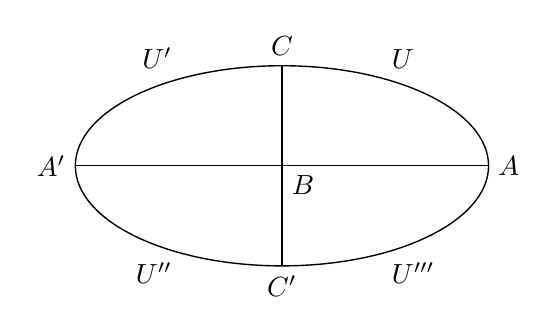
\begin{tikzpicture}[scale=0.82,line width=0.5pt]
  \draw (0,0) ellipse (3.2 and 1.55);
  \draw (-3.2,0) -- (3.2,0);
  \draw (0,-1.55) -- (0,1.55);
  \node[left] at (-3.2,0) {$A'$};
  \node[right] at (3.2,0) {$A$};
  \node[above] at (0,1.55) {$C$};
  \node[below] at (0,-1.55) {$C'$};
  \node[below right] at (0,0) {$B$};
  \node[above left] at (-1.55,1.35) {$U'$};
  \node[above right] at (1.55,1.35) {$U$};
  \node[below left] at (-1.55,-1.35) {$U''$};
  \node[below right] at (1.55,-1.35) {$U'''$};
\end{tikzpicture}
\end{center}

32. Hence, in order that the equation
\[
 dp\sqrt{\frac{p}{(a+p)(b+p)(c+p)(\theta+p)}}
 \pm dq\sqrt{\frac{q}{(a+q)(b+q)(c+q)(\theta+q)}}=0
\]
of the geodesic lines may be real (observing that we have
$a+p,b+p=+,c+p,p=-$, and $a+q=+,b+q,c+q,q=-$, consequently
$p\div(a+p)(b+p)(c+p)=+$, but $q\div(a+q)(b+q)(c+q)=-$), we must have
$\theta+p,\theta+q$ of opposite signs, that is $\theta+p=+$ and $\theta+q=-$; or $\theta$
included between the limits $a,c$. Or, what is the same thing, $-\theta$ is included between
the limits $-c,-b$, say $-\theta$ has a $p$-value; or else between the limits $-b,-a$,
say $-\theta$ has a $q$-value. This is conveniently shown in the annexed diagram of the
values of $-p,-q,-\theta$.

\begin{center}
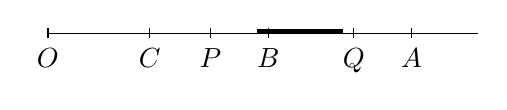
\begin{tikzpicture}[x=0.7cm,y=0.7cm,line width=0.5pt]
  \draw (-4,0) -- (3.8,0);
  \foreach \x/\lab in {-4/O,-2.15/C,-1.05/P,0/B,1.55/Q,2.6/A} {
    \draw (\x,0.09) -- (\x,-0.09);
    \node[below] at (\x,-0.09) {$\lab$};
  }
  \draw[line width=1.3pt] (-0.2,0.04) -- (1.35,0.04);
\end{tikzpicture}
\end{center}

Hence on the ellipsoid we have two kinds of geodesic lines, each of them touching a real
curve of curvature; viz. those which touch a major-mean curve and those which touch a
minor-mean curve: the transition case, answering to the value $\theta=b$, is that of the
geodesic lines which pass through an umbilicus. I have considered the theory more in detail
in my memoir ``On the Geodesic Lines of an Ellipsoid,'' \emph{Mem. R. Ast. Soc.}, t. xxx.,
pp. 31--53, 1872, [478].

33. Next, for the skew hyperboloid, we have $a$ and $b=+$, $c=-$, and I assume for
convenience $a>b$. Attending to the signs, we still have therefore $a>b>c$. The principal
sections are one of them an ellipse, and the other two hyperbolas, viz. the minor section is
the ellipse $\frac{x^2}{a}+\frac{y^2}{b}=1$, the major section is the hyperbola
$\frac{y^2}{b}+\frac{z^2}{c}=1$, and the mean section is the hyperbola
$\frac{x^2}{a}+\frac{z^2}{c}=1$: there are no umbilici. The elliptic coordinates enter
symmetrically; but, as before, we distinguish them, viz. we take $p$ to extend from $-c$
(a positive value) to infinity, and $q$ from $-b$ to $-a$. Thus $p=\mathrm{const.}$ denotes
the curves of curvature of the one kind, viz. $p=-c$ the ellipse
$\frac{x^2}{a}+\frac{y^2}{b}=1$, and every other value of $p$ an oval curve surrounding the
hyperboloid; and $q=\mathrm{const.}$ the curves of curvature of the other kind, viz.
$q=-c$ the major hyperbola $\frac{y^2}{b}+\frac{z^2}{c}=1$, $q=-b$ the mean hyperbola
$\frac{x^2}{a}+\frac{z^2}{c}=1$, and each intermediate value gives a curve of curvature
of a hyperbolic form: we may say that $p=\mathrm{const.}$ determines the oval curves of
curvature, and $q=\mathrm{const.}$ the hyperbolic curves of curvature.

34. In the equation of the geodesic lines we have $a+p,b+p,c+p,p$ all positive; but
$a+q=+,b+q,c+q,q$ each $=-$; thence
$p\div(a+p)(b+p)(c+p)=+$, but $q\div(a+q)(b+q)(c+q)=-$; therefore $\theta+p$ and
$\theta+q$ must be of opposite signs, or we must have $\theta+p=+$ and $\theta+q=-$;
or what is the same thing, $\theta$ may have any value from $-p$ to $-q$, or say
$-\theta$ any value from $p$ to $q$; that is, the value of $-\theta$ may be positive and
greater than $-c$, positive and less than $-c$, negative and less than $-b$, negative and
between $-b$ and $-a$; viz. in the first case $-\theta$ has a $p$-value, and in the fourth
case it has a $q$-value, but in the second and third cases it has neither a $p$- nor a
$q$-value. This is better seen from the diagram.

\begin{center}
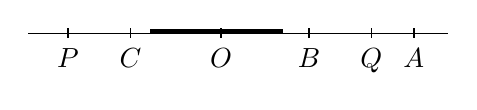
\begin{tikzpicture}[x=0.72cm,y=0.7cm,line width=0.5pt]
  \draw (-3.4,0) -- (4.0,0);
  \foreach \x/\lab in {-2.7/P,-1.6/C,0/O,1.55/B,2.65/Q,3.4/A} {
    \draw (\x,0.09) -- (\x,-0.09);
    \node[below] at (\x,-0.09) {$\lab$};
  }
  \draw[line width=1.3pt] (-1.25,0.04) -- (1.1,0.04);
\end{tikzpicture}
\end{center}

It follows that we have, on the hyperboloid, geodesic lines of four different kinds:
those which touch a real curve of curvature, oval or hyperbolic, and those which touch no
real curve of curvature, but for which $-\theta$ has a positive value from $0$ to $-c$, or
a negative value from $0$ to $-b$. And there are the transitional cases $-\theta=-c$,
where the geodesic touches the ellipse $\frac{x^2}{a}+\frac{y^2}{b}=1$; $\theta=0$,
where the geodesic becomes a right line; and $-\theta=-b$, where the geodesic touches the
mean hyperbola $\frac{x^2}{a}+\frac{z^2}{c}=1$.

35. To explain this more in detail, consider the geodesics which start from a point $M$ of
the hyperboloid. To fix the ideas, consider the axis of $z$ as vertical, and take the point
$M$ in the positive octant of the hyperboloid; and let $M1$ represent the direction of the
oval curve of curvature, $M9$ that of the hyperbolic curve of curvature, $M5$ that of one
of the right lines.

The geodesic of initial direction $M1$ touches at $M$ the oval curve of curvature $M1$,
and lies wholly above this curve; it makes an infinity of convolutions round the upper part
of the hyperboloid, cutting all the oval curves of curvature for which $p$ has a positive
value greater than $p_1$ (if $p_1$ is the value of $p$ corresponding to the oval curve
through $M$), and ascending to infinity: or considering the curve as described in the opposite
sense, it descends from infinity to touch the oval curve through $M$, after which it again
ascends to infinity.

\begin{center}
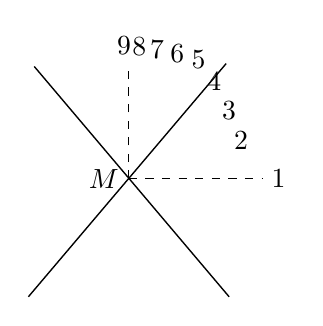
\begin{tikzpicture}[scale=0.75,line width=0.5pt]
  \draw (-1.6,1.9) -- (1.7,-2.0);
  \draw (-1.7,-2.0) -- (1.65,1.95);
  \draw[dashed] (0,0) -- (2.25,0);
  \draw[dashed] (0,0) -- (0,1.9);
  \node[left] at (0,0) {$M$};
  \node[right] at (2.25,0) {$1$};
  \node at (1.9,0.65) {$2$};
  \node at (1.7,1.15) {$3$};
  \node at (1.45,1.65) {$4$};
  \node at (1.18,2.02) {$5$};
  \node at (0.82,2.12) {$6$};
  \node at (0.48,2.18) {$7$};
  \node at (0.18,2.23) {$8$};
  \node at (-0.08,2.25) {$9$};
\end{tikzpicture}
\end{center}

Next, if the initial direction is $M2$, we have a geodesic of the same kind, only descending
below $M$ to touch a certain oval curve having for its parameter $p_2$ $(p_2>-c<p_1)$.

We come next to a critical direction $M3$, for which the geodesic descends below $M$ to
touch the oval curve of parameter $p_3=-c$, that is, the ellipse
$\frac{x^2}{a}+\frac{y^2}{b}=1$. But it is to be observed that, whatever the initial point
$M$ may be, the geodesic makes below $M$ an infinity of convolutions round the hyperboloid,
so that it does not in fact ever actually touch the ellipse, but has this ellipse for an
asymptote. That this is so appears from the consideration that the ellipse, \emph{qua} plane
curve of curvature, is a geodesic; so that, starting from a point of the ellipse in the
direction of the ellipse, the geodesic coincides with the ellipse, or, besides the ellipse
itself, there is not any geodesic which touches the ellipse.

Next, if the initial direction be $M4$, the geodesic does not here touch any oval curve;
it descends through $M$ below the ellipse $\frac{x^2}{a}+\frac{y^2}{b}=1$, lying in the
upper and lower portions of the hyperboloid, and making round it an infinity of convolutions.

36. We come, then, to the initial direction $M5$, which is that of the right line; the
geodesic here coincides with the right line.

In the cases which follow, the geodesic lies in the upper and lower portions of the
hyperboloid, cutting all the oval curves of curvature.

Initial direction $M6$: the geodesic does not touch any hyperbolic curve of curvature, but
makes round the hyperboloid an infinity of convolutions.

Initial direction $M7$: the geodesic touches at opposite infinities the mean hyperbola
$\frac{x^2}{a}+\frac{z^2}{c}=1$, it lies wholly in front of the plane $y=0$ of this hyperbola.

Initial direction $M8$: the geodesic touches a hyperbolic curve of curvature parameter
$q_8$ where $q_8$ (negative) is between $-b$ and $q_9$ the parameter of the hyperbolic
curve of curvature through $M$; viz. it cuts all the hyperbolic curves the parameters of
which are between $-b$ and $q_8$, but does not cut the remaining curves the parameters of
which extend from $q_8$ to $-a$.

Lastly, initial direction is $M9$, that of the hyperbolic curve of curvature through $M$;
the geodesic touches this curve, cutting all the hyperbolic curves the parameters of which
are between $-b$ and $q_9$, but not any of those the parameters of which are between $q_9$
and $-a$.

37. If in the differential equation of the geodesic line we consider $p,q$ as the elliptic
coordinates of a given point $M$ of the curve, the equation for a given value of $\theta$
determines the direction of the curve; or conversely, if the direction be given, the equation
determines the value of the parameter $\theta$. Writing
\[
 \frac{dp\sqrt p}{\sqrt{(a+p)(b+p)(c+p)}}=P,\qquad
 \frac{dq\sqrt q}{\sqrt{(a+q)(b+q)(c+q)}}=Q,
\]
then $P,Q$ are proportional to the rectangular coordinates of a consecutive point $M'$,
measured from $M$ in the directions of the hyperbolic and oval curves of curvature
respectively; and the differential equation of the geodesic lines gives
\[
 \frac{P}{\sqrt{p+\theta}}\pm\frac{Q}{\sqrt{q+\theta}}=0;
\]
viz. if $\phi$ be the inclination of the geodesic to the hyperbolic curve of curvature,
then $Q=P\tan\phi$, or we have
\[
 \frac{1}{p+\theta}=\frac{\tan^2\phi}{q+\theta},
\]
that is, $p\tan^2\phi-q=\theta(1-\tan^2\phi)$; hence, if for the right line $\phi=\lambda$,
then $p\tan^2\lambda-q=0$; and therefore
\[
 \theta=\frac{p(\tan^2\phi-\tan^2\lambda)}{1-\tan^2\phi},
\]
viz. $\phi=0$, $\theta=-q$, $=\infty$, $\theta=-p$, as it should be.

\paperid{509}
\section*{509. Plan of a Curve-Tracing Apparatus}

\begin{center}
{\small [From the \emph{Proceedings of the London Mathematical Society}, vol. iv. (1871--1873),
pp. 345--347. Read May 8, 1873.]}
\end{center}

I have devised a curve-tracing apparatus on the following plan:

Imagine two planes $\Pi,\Pi'$ moving in the same horizontal plane, and above the two planes
respectively the two points $P,P'$ moving in the same or a parallel plane.

To fix the ideas, suppose that the two planes each move according to a law (that is, let the
motion of each of them depend on a single variable parameter; for instance, they may each of
them rotate about an axis); but let the motion of the two points be free.

Suppose, next, that the planes are connected together in such manner that the motion of one
of them determines the motion of the other (e.g. by a train of wheel-work); and that the two
points are also connected together in such manner that the motion of one of them determines
the motion of the other (e.g. by a pentagraph, or by a slotted rod, the slot of which works
on an axle, so as to allow the rod to move lengthways as well as rotate).

Suppose, finally, that one of the points, say $P'$, is attached to a point of the plane
$\Pi'$; then the plane $\Pi$ being set in motion, this determines the motion of $\Pi'$,
consequently of $P'$, consequently of $P$; and the moving point $P$, or say the pencil $P$,
will describe on the moving plane $\Pi$ a curve, the nature of which will of course depend
on the nature of the motions of $\Pi,\Pi'$, and on that of the connection between these
planes and of the connections between the points $P$ and $P'$.

I propose to describe the apparatus as nearly as I have actually constructed it. (See
sketch-plan Fig. 1, and side-elevation Fig. 2.)

The framework of the instrument consists of two longitudinal bars ($B$) each about three
feet long, one inch thick, and three inches broad, supported edgewise at a distance of about
eighteen inches on the cross-pieces $C,C$; and half-way between them, supported by the same
cross-pieces, is an axis carrying at each extremity two mitre wheels. The bars $B$ support
three cross-pieces $D,D,D$, and between these are the moveable cross-pieces $E,E$ carrying
the axes $A,A$ with the attached mitre wheels, and circular disks $X,X$. Each of these
wheels separately may be placed (as in the figure) out of gear with the two vertical wheels,
or it can (by moving the cross-piece $E$) be brought into gear with either of these wheels.
Each axis $A$ passes through a circular disk $H$, capable of rotating about it, so that it may
be fixed in any position, and serving as the bearing for the plane $X$.

\begin{center}
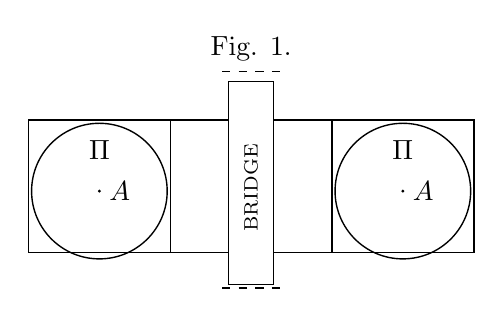
\begin{tikzpicture}[scale=0.82,line width=0.5pt]
  \node at (0,2.35) {Fig. 1.};
  \draw[dashed] (-0.45,2.0) -- (0.45,2.0);
  \draw[dashed] (-0.45,-1.35) -- (0.45,-1.35);
  \draw (-0.35,-1.3) rectangle (0.35,1.85);
  \node[rotate=90] at (0,0.2) {\scriptsize BRIDGE};
  \foreach \x in {-2.35,2.35} {
    \draw (\x-1.1,-0.8) rectangle (\x+1.1,1.25);
    \draw (\x,0.15) circle (1.05);
    \node at (\x,0.78) {$\Pi$};
    \fill (\x,0.15) circle (0.025);
    \node[right] at (\x,0.15) {$A$};
    \draw (\x+1.1,1.25) -- ({ifthenelse(\x<0,-0.35,0.35)},1.25);
    \draw (\x+1.1,-0.8) -- ({ifthenelse(\x<0,-0.35,0.35)},-0.8);
  }
\end{tikzpicture}
\end{center}

The disks $X,X$ may be regarded as being themselves the planes $\Pi,\Pi$ (say these planes
are rigidly attached to $X,X$ respectively); or we may, in any other manner, move the plane
$\Pi$ by means of the disk $X$; for instance, $X$ may carry a spur-wheel gearing into a
spur-wheel on the under surface of $\Pi$, and thereby communicating a rotation of different
velocity to the plane $\Pi$; or the connection may be as in the ordinary oval chuck. In any
such case, the disk $H$ (which, for this reason, was made to project beyond $X$) serves as
a support for the plane $\Pi$, and the apparatus connected therewith; and observe that the
angular position of such apparatus, and therefore of the path of any point of $\Pi$, may be
varied at pleasure by moving the disk $H$ through any angle.

\begin{center}
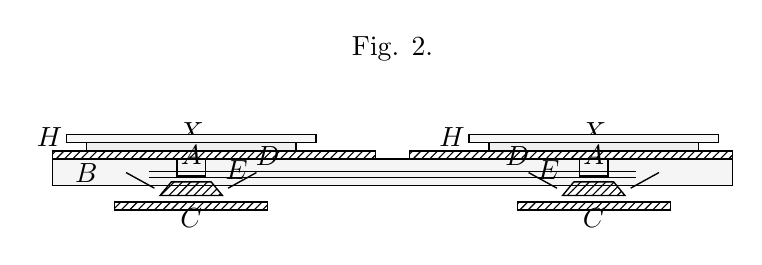
\begin{tikzpicture}[x=0.72cm,y=0.62cm,line width=0.5pt]
  \node at (0,2.25) {Fig. 2.};
  \draw[fill=gray!8] (-6,-0.55) rectangle (6,0);
  \node at (-5.4,-0.3) {$B$};
  \draw[pattern=north east lines] (-6,0.0) rectangle (-0.3,0.16);
  \draw[pattern=north east lines] (0.3,0.0) rectangle (6,0.16);
  \foreach \x in {-3.55,3.55} {
    \draw[fill=gray!12] (\x-1.85,0.16) rectangle (\x+1.85,0.34);
    \node at (\x,0.55) {$X$};
    \draw[fill=gray!6] (\x-2.2,0.34) rectangle (\x+2.2,0.50);
    \node at (\x-2.5,0.45) {$H$};
    \draw (\x-0.25,0) rectangle (\x+0.25,-0.35);
    \node at (\x,0.07) {$A$};
    \draw[pattern=north east lines] (\x-0.55,-0.75) -- (\x+0.55,-0.75) -- (\x+0.35,-0.47) -- (\x-0.35,-0.47) -- cycle;
    \draw (\x-0.65,-0.6) -- (\x-1.15,-0.28);
    \draw (\x+0.65,-0.6) -- (\x+1.15,-0.28);
    \draw[pattern=north east lines] (\x-1.35,-1.05) rectangle (\x+1.35,-0.88);
    \node at (\x,-1.22) {$C$};
  }
  \draw (-4.3,-0.26) -- (4.3,-0.26);
  \draw (-4.3,-0.38) -- (4.3,-0.38);
  \node at (-2.2,0.06) {$D$};
  \node at (2.2,0.06) {$D$};
  \node at (-2.75,-0.22) {$E$};
  \node at (2.75,-0.22) {$E$};
\end{tikzpicture}
\end{center}

Detached altogether from the rest of the instrument, or what is better, supported on
longitudinal pieces carried by the cross-pieces $C,C$ we have a bridge (see fig. 1) capable
of adjustment as regards height, and serving as a support for the pentagraph-apparatus, or
other connection of the one plane $\Pi$ with the pencil which works upon the other plane
$\Pi$.

It is hardly necessary to remark that in the simple form of the instrument where the disks
$X,X$ are themselves the planes $\Pi,\Pi$, then putting the mitre wheel of one plane $X$
in gear with either of the corresponding vertical wheels, and making the plane rotate, the
other plane $X$ will rotate with the same angular velocity, in the same or the opposite
direction, or it will remain at rest, according as its mitre wheel is in gear with one or
the other of the corresponding vertical wheels, or is out of gear with each of them.

\paperid{510}
\section*{510. On Bicursal Curves}

\begin{center}
{\small [From the \emph{Proceedings of the London Mathematical Society}, vol. iv. (1871--1873),
pp. 347--352. Read May 8, 1873.]}
\end{center}

A curve of deficiency 1 may be termed bicursal; there is some distinction according as the
order is even or odd, and to fix the ideas I take it to be even.

A bicursal curve of the order $n$ contains
\[
 \frac12 n(n+3)-\left\{\frac12(n-1)(n-2)-1\right\}=3n
\]
constants; hence, if the order is $=2n$, the number of constants is $=6n$; such a curve is
normally represented by a system of equations
\[
 (x,y,z)=(1,\theta)^n+(1,\theta)^{n-2}\sqrt\Theta,
\]
where $\Theta$ is a quartic function, which may be taken to be of the form
$(1-\theta^2)(1-k^2\theta^2)$, or otherwise to depend on a single constant; viz.
$(x,y,z)$ are proportional to $n$-thic functions involving such a radical: since in the
values of $(x,y,z)$ one constant divides out, the number of constants is
$3\{(n+1)+(n-1)\}-1+1=6n$, as it should be.

But the curve of the order $2n$ may be abnormally or improperly represented by a system of
equations
\[
 (x,y,z)=(1,\theta)^{n+k}+(1,\theta)^{n+k-2}\sqrt\Theta,
\]
viz. these equations, instead of representing a curve of the order $2n+2k$, will represent
a curve of the order $2n$, provided only there exist $2k$ common values of $\theta$ for which
each of the three functions vanish. The passage to a normal representation is effected by
finding $\theta'$ a function of $\theta,\sqrt\Theta$ (viz. an irrational function of $\theta$)
such that the foregoing equations become
\[
 (x,y,z)=(1,\theta')^n+(1,\theta')^{n-2}\sqrt{\Theta'};
\]
it is shown that such a transformation is possible, and a mode of effecting it, derived from
a theorem of Hermite's in relation to the Jacobian $H,\Theta$ functions, is given in Clebsch's
Memoir ``Ueber diejenigen Curven, deren Coordinaten sich als elliptische Functionen eines
Parameters darstellen lassen,'' \emph{Crelle}, t. LXIV. (1865), pp. 210--270. The
demonstration is a very interesting one, and I reproduce it at the end of this paper. I remark,
in passing, that the analogous reduction in the case of unicursal curves is self-evident;
the equations
\[
 (x,y,z)=(1,\theta)^{n+k}
\]
will represent a curve, not of the order $n+k$, but of the order $n$, provided there exist
$k$ common values of $\theta$ for which the three functions vanish; in fact, the three
functions have then a common factor of the order $k$, and omitting this, the form is
$(x,y,z)=(1,\theta)^n$.

Returning to the curves of deficiency 1, we see that a curve of the order $2m+2n$ contains
$6(m+n)$ constants, and is normally represented by a system of equations
\[
 (x,y,z)=(1,\theta)^{m+n}+(1,\theta)^{m+n-2}\sqrt\Theta.
\]
Such a curve may be otherwise represented: we may derive it by a rational transformation
from the curve $(D=1)$ of the order 4 (binodal quartic), the equation of which is
\[
 (1,u)^2(1,v)^2=0;
\]
viz. the coordinates are here connected by a quadriquadric equation; and we then express
$x,y,z$ in terms of these by a system of equations
\[
 (x,y,z)=(1,u)^m(1,v)^n.
\]

It is, however, to be observed that the form of these functions is not determinate: each of
them may be altered by adding to it a term
$(1,u)^{m-2}(1,v)^{n-2}\{(1,u)^2(1,v)^2\}$, where the second factor is that belonging to the
quadriquadric transformation, and the first factor is arbitrary. Using the arbitrary function
to simplify the form, the real number of constants is reduced to
$(m+1)(n+1)-(m-1)(n-1)=2(m+n)$; or the three functions contain together $6(m+n)$ constants,
one of which divides out. The quadriquadric equation, dividing out one constant, contains
eight constants; but reducing by linear transformations on $u,v$ respectively, the number of
constants is $8-6=2$. Hence, in the system of equations, the whole number of constants is
$6(m+n)-1+2=6(m+n)+1$; viz. this is greater by unity than the number of constants in the
curve $(D=1)$ of the order $2(m+n)$. The explanation of the excess is that the same curve of
the order $2(m+n)$ may be derived from the different quartic curves
$(1,u)^2(1,v)^2=0$; this will be further examined.

The transition from the one form to the other is not immediately obvious; in fact, if from
the quadriquadric equation $(1,u)^2(1,v)^2=0$ (say this is
$A+2Bv+Cv^2=0$, where $A,B,C$ are quadric functions of $u$) we determine $v$; this gives
$Cv=-B+\sqrt{B^2-AC}$, $=-B+\sqrt\Omega$ suppose; and then substituting in the equations
$(x,y,z)=(1,u)^m(1,v)^n$, we find
\[
 (x,y,z)=(1,u)^m(C,-B+\sqrt\Omega)^n;
\]
viz. we have $(x,y,z)$ proportional to functions of $u$, involving the quartic radical
$\sqrt\Omega$; but these functions are of the order (not $m+n$, but) $m+2n$.

In particular, if $n=m$, then, instead of functions of the order $2n$, we have functions
of the order $3n$. The reduction in this last case to the form where the order is $2n$ can
be effected without difficulty, but in the general case where $m$ and $n$ are unequal, I do
not know how it is to be effected except by the general process explained in Clebsch's
Memoir.

We may, in fact, by linear transformations on $u,v$, reduce the quadriquadric relation to
\[
\begin{matrix}
1&+u^2\\
&+2buv\\
+v^2&+cu^2v^2=0,
\end{matrix}
\]
that is
\[
 1+u^2+2buv+v^2+cu^2v^2=0;
\]
or putting herein $u+v=p$, $uv=q$, the relation is
\[
 1+p^2-2q+2bq+cq^2=0,
\]
that is
\[
 p^2=-1+(2-2b)q-cq^2,\qquad
 p^2-4q=-1+(-2-2b)q-cq^2;
\]
viz. extracting the square roots,
\[
 u+v=\sqrt Q,\qquad u-v=\sqrt{Q'},
\]
if for shortness
\[
 Q=-1+(2-2b)q-cq^2,\qquad Q'=-1+(-2-2b)q-cq^2;
\]
we may then rationalise one of the radicals, for instance $Q$; viz. writing
\[
 -c\{-1+(2-2b)q-cq^2\}=\{cq-(1-b)\}^2+c-(1-b)^2,
\]
then, if
\[
 cq-(1-b)=\sqrt{c-(1-b)^2}\cdot\frac12\left(\theta-\frac{1}{\theta}\right),
\]
this becomes
\[
 -cQ=\{c-(1-b)^2\}
 \left\{\frac14\left(\theta-\frac{1}{\theta}\right)^2+1\right\}
 =\{c-(1-b)^2\}\cdot\frac14\left(\theta+\frac{1}{\theta}\right)^2,
\]
that is
\[
 \sqrt Q=\frac12\sqrt{\frac{c-(1-b)^2}{-c}}\left(\theta+\frac{1}{\theta}\right);
\]
and the corresponding value of $\sqrt{Q'}$ is
\[
 \sqrt{Q'}=
 \sqrt{\frac14\frac{c-(1-b)^2}{-c}\left(\theta+\frac{1}{\theta}\right)^2-4q},
\]
where $q$ stands for its value
\[
 \frac1c\left\{1-b+\sqrt{c-(1-b)^2}\cdot\frac12\left(\theta-\frac{1}{\theta}\right)\right\}.
\]
We may write these in the form
\[
 1:\frac12\sqrt Q:\frac12\sqrt{Q'}=M\theta:1+\theta^2:\sqrt\Theta,
\]
where $M$ is a constant, and $\Theta$ is a quartic function of $\theta$, such that
$(1+\theta^2)^2-\Theta$ is a quadric function only of $\theta$.

The equations
\[
 (x,y,z)=(1,u)^m(1,v)^n
\]
thus assume the form
\[
 (x,y,z)=(M\theta,1+\theta^2+\sqrt\Theta)^m
 (M\theta,1+\theta^2-\sqrt\Theta)^n;
\]
and on the right-hand side the term of the highest order in $\theta$ is
\[
 (1+\theta^2+\sqrt\Theta)^m(1+\theta^2-\sqrt\Theta)^n,
\]
viz. if $n=$ or $>m$, then this is
\[
 \{(1+\theta^2)^2-\Theta\}^m(1+\theta^2-\sqrt\Theta)^{n-m}.
\]
This is
\[
 =(1,\theta)^{2m}(1+\theta^2-\sqrt\Theta)^{n-m},
\]
which is of the order $2m+2(n-m)=2n$ (which, in virtue of $n=$ or $>m$, is $=$ or
$>m+n$). In particular, if $n=m$, then the highest order is $=2n$; or the curve of the
order $2n$, as represented by the equations
\[
 (x,y,z)=(1,u)^n(1,v)^n,
\]
where $(u,v)$ are connected by a quadriquadric equation, is also represented by the equations
\[
 (x,y,z)=(1,\theta)^n+(1,\theta)^{n-2}\sqrt\Theta,
\]
which is the required transformation of the original equations.

It is to be noticed that the foregoing form,
\[
\begin{matrix}
1&+u^2\\
&+2buv\\
+v^2&+cu^2v^2=0,
\end{matrix}
\]
is the most special form to which the quadriquadric relation can be reduced by the linear
transformations of $u,v$; in fact, by mere division, the equation is made to have the constant
term 1; the number of the coefficients of transformation is then $3+3=6$; and to reduce the
relation to the foregoing form, we have the six conditions, coeff. $u=0$, coeff. $v=0$,
coeff. $uv^2=0$, coeff. $v^2u=0$, coeff. $u^2=1$, coeff. $v^2=1$; but in this form,
expressing $v$ in terms of $u$, the radical is $\sqrt\Omega$, where
\[
 \Omega=(1+u^2)(1+cu^2)-b^2u^2,
\]
which is not more general than if we had
\[
 \Omega=(1+u^2)(1+cu^2),
\]
viz. there is a superfluous constant $b$. And we thus see how it is that the system of
equations
\[
 (x,y,z)=(1,u)^n(1,v)^n,
\]
$(u,v)$ connected by a quadriquadric relation, contains, not $6n$, but $6n+1$ constants,
one of these being superfluous.

Clebsch's transformation, above referred to, is as follows:

Starting with the equations
\[
 (x,y,z)=(1,\theta)^{n+k}+(1,\theta)^{n+k-2}\sqrt\Theta,
\]
if the function $\Theta$ is not originally of the standard form, we may, by a linear
substitution, reduce it to this form, viz. we may write
\[
 \Theta=\theta(1-\theta)(1-k^2\theta);
\]
and then writing $\theta=\sn^2u$, $(\sin^2\operatorname{am}u)$, we have
\[
 \sqrt\Theta=\sn u\,\cn u\,\dn u=\sn u\,\sn' u;
\]
so that the formulae become
\[
 (x,y,z)=(1,\sn^2u)^{n+k}+(1,\sn^2u)^{n+k-2}\sn u\,\sn' u.
\]

Hermite's theorem, used in the demonstration, is that any such function of $\sn u$ is
expressible in the form
\[
 C\,\frac{H(u-\alpha_1)H(u-\alpha_2)\cdots H(u-\alpha_{2n+2k})}{\Theta^{2n+2k}(u)}
\]
($H,\Theta$ denoting here the two Jacobian functions), where
\[
 \alpha_1+\alpha_2\cdots+\alpha_{2n+2k}=0.
\]
Observe, in passing, that the equation
\[
 0=(1,\sn^2u)^{n+k}+(1,\sn^2u)^{n+k-2}\sn u\,\sn' u
\]
gives, when rationalised, an equation in $\sn^2u$ of the order $2n+2k$; its roots are
\[
 \sn^2\alpha_1,\ \sn^2\alpha_2,\ \ldots,\ \sn^2\alpha_{2n+2k}.
\]
Considering the
functions $(1,\sn^2u)^{n+k}$ and $(1,\sn^2u)^{n+k-2}$ as indeterminate, the coefficients can
be found so that all but one of the roots of the equation in $\sn^2u$ shall have any given
values whatever,
\[
 \sn^2\alpha_1,\ \sn^2\alpha_2,\ \ldots,\ \sn^2\alpha_{2n+2k-1};
\]
the theorem then
shows that the remaining root is $\sn^2\alpha_{2n+2k}$, where
\[
 -\alpha_{2n+2k}=\alpha_1+\alpha_2\cdots+\alpha_{2n+2k-1},
\]
which is, in fact, Abel's theorem.

Now, supposing that the three functions of $\theta$ all vanish for $2k$ common values of
$\theta$, each of the functions of $u$ will contain the same $2k$ $H$ functions, say these
are $H(u-\alpha_{2n+1})\cdots H(u-\alpha_{2n+2k})$. Omitting these and also the denominator
factor $\Theta^{2k}(u)$, we have the set of equations
\[
 (x,y,z)=C\,\frac{H(u-\alpha_1)H(u-\alpha_2)\cdots H(u-\alpha_{2n})}{\Theta^{2n}(u)},
\]
where, however,
\[
 \alpha_1+\alpha_2\cdots+\alpha_{2n}\ne0,
\]
the values $\alpha_1,\alpha_2,\ldots,\alpha_{2n}$ are of course different for the three
coordinates $x,y,z$ respectively; viz. we have
\[
 \alpha_1+\alpha_2\cdots+\alpha_{2n}
 =-(\alpha_{2n+1}+\cdots+\alpha_{2n+2k})=2ns\quad\hbox{suppose.}
\]
Writing then
\[
 u=u'+s,\quad \alpha_1=\alpha'_1+s,\quad \alpha_2=\alpha'_2+s,\ldots,\quad
 \alpha_{2n}=\alpha'_{2n}+s,
\]
and consequently
\[
 \alpha'_1+\alpha'_2+\cdots+\alpha'_{2n}=0,
\]
we have
\[
 (x,y,z)=C\,\frac{H(u'-\alpha'_1)\cdots H(u'-\alpha'_{2n})}{\Theta^{2n}(u'+s)};
\]
or, changing the common denominator,
\[
 (x,y,z)=C\,\frac{H(u'-\alpha'_1)\cdots H(u'-\alpha'_{2n})}{\Theta^{2n}(u')},
\]
where
\[
 \alpha'_1+\alpha'_2\cdots+\alpha'_{2n}=0;
\]
or, what is the same thing,
\[
 (x,y,z)=(1,\sn^2u')^n+(1,\sn^2u')^{n-2}\sn u'\,\sn' u';
\]
viz. writing $\sn u'=\theta'$, and $\Theta'=\theta'(1-\theta')(1-k^2\theta')$, this is
\[
 (x,y,z)=(1,\theta')^n+(1,\theta')^{n-2}\sqrt{\Theta'},
\]
a normal representation of the curve of the order $2n$.

The relation between the parameters $\theta,\theta'$ is given by
$\theta'=\sn^2(u-s)$, $\sn^2u=\theta$, that is, we have
\[
 \sqrt{\theta'}=
 \frac{\sqrt\theta\,\cn s\,\dn s-\sn s\sqrt{(1-\theta)(1-k^2\theta)}}
 {1-k^2\sn^2s\,\theta};
\]
or, writing $\sn^2s=\sigma$, this is
\[
 \theta'=
 \frac{\sqrt\theta\sqrt{(1-\sigma)(1-k^2\sigma)}
 -\sqrt\sigma\sqrt{(1-\theta)(1-k^2\theta)}}{1-k^2\sigma\theta};
\]
and, conversely, we have
\[
 \theta=
 \frac{\sqrt{\theta'}\sqrt{(1-\sigma)(1-k^2\sigma)}
 +\sqrt\sigma\sqrt{(1-\theta')(1-k^2\theta')}}
 {1-k^2\sigma\theta'},
\]
and the theorem, in fact, shows that, substituting this value of $\theta$ in the functions
of $\theta$ which serve to express $x,y,z$, these become \emph{proportional} to the functions
of $\theta'$; viz. they become equal to these functions, each multiplied by an irrational
function $A'+B'\sqrt{\Theta'}$, ($A',B'$ rational functions of $\theta'$).

\paperid{511}
\section*{511. Addition to the Memoir on Geodesic Lines, in particular those of a Quadric Surface (509)}

\begin{center}
{\small [From the \emph{Proceedings of the London Mathematical Society}, vol. iv. (1871--1873),
pp. 368--380. Read June 12, 1873.]}
\end{center}

38. In the Memoir above referred to, speaking of the geodesic lines on the skew hyperboloid,
I say (No. 35), ``The geodesic of initial direction $M1$ touches at $M$ the oval curve of
curvature $M1$, and lies wholly above this curve; it makes an infinity of convolutions round
the upper part of the hyperboloid, cutting all the oval curves of curvature for which $p$ has
a positive value greater than $p_1$ (if $p_1$ is the value of $p$ corresponding to the oval
curve through $M$), and ascending to infinity.'' The statement as to the infinity of
convolutions is incorrect; I was led to it by the assumption that the geodesic could not touch
any hyperbolic curve of curvature. The fact is, that it touches at infinity (has for
asymptotes) in general two hyperbolic curves of curvature; viz. the geodesic descending from
infinity in the direction of a hyperbolic curve of curvature, so as to touch the oval curve
through $M$, again ascends to infinity in the direction of a hyperbolic curve of curvature
(the same as the first-mentioned one, or a different curve), making in its whole course say
$k$ convolutions, where $m$ is a positive finite number; if $k<1$, there is no complete
convolution, and when $k=1$ or any integer number, then the two hyperbolic curves are one
and the same curve; $k$ is infinite only in the special case afterwards referred to in the
same No. 35, where the oval curve of curvature is the ellipse which is a principal section
of the hyperboloid, and does not even attain to the value 1 except for an oval curve
exceedingly close to this ellipse. The error was on consideration obvious enough, though
I was in fact led to perceive it by the numerical calculations about to be referred to, which
gave me geodesics not making a complete convolution.

\begin{center}
{\footnotesize $^1$ The articles are numbered consecutively with those of the Memoir, (509).}
\end{center}

39. I have effected, for a particular skew hyperboloid and oval curve of curvature thereof,
the numerical calculations for laying down the geodesic lines which touch this curve of
curvature. Taking in general the equation of the hyperboloid to be
\[
 \frac{x^2}{a}+\frac{y^2}{b}+\frac{z^2}{c}=1,
\]
and the $\theta$-curve of curvature to be the intersection by the confocal surface
\[
 \frac{x^2}{a-\theta}+\frac{y^2}{b-\theta}+\frac{z^2}{c-\theta}=1,
\]
then the selected values for the hyperboloid, and oval curve of curvature touched by the
geodesics, are
\[
 a=900,\qquad b=400,\qquad c=-c'=-1600,\qquad \theta=-\theta'=-1650;
\]
so that $a,b,c',\theta'$ are the positive values $900,400,1600$, and $1650$ respectively.
I recall that $p=c'$ to $p=\infty$ gives the oval curves of curvature, viz. $p=c'$, the
elliptic principal section; $p=\theta'$, the given oval curve: and that we are in the sequel
concerned only with the oval curves above this, for which $p$ extends from $\theta'$ to
$\infty$. Moreover, $q=-b$ to $-a$ gives the hyperbolic curves of curvature, viz.
$q=-b$ the $xz$-principal section; and $q=-a$ the $yz$-principal section of the hyperboloid.
We have, in fact, to deal with the integrals
\[
 \Pi(p)=\int_{\theta'}^p dp\,
 \sqrt{\frac{p}{(p+a)(p+b)(p-c')(p-\theta')}},
\]
\[
 \Psi(q)=\int_{-b}^{q} dq\,
 \sqrt{\frac{q}{(q+a)(q+b)(q-c')(q-\theta')}},
\]
or if $p=\theta'+u$, $u$ extending from 0 towards $\infty$, then
\[
 \Pi(p)=\int_0^u du\,
 \sqrt{\frac{u+\theta'}{(u+a+\theta')(u+b+\theta')(u+\theta'-c')u}},
\]
and so if $q=-b-v$, $v$ extending from 0 towards $(a-b)$, which is its limit,
\[
 \Psi(q)=\int_0^v dv\,
 \sqrt{\frac{v+b}{(a-b-v)v(v+b+c')(v+b+\theta')}}.
\]
The relation for any particular geodesic of the series being
\[
 \pm\Pi(p)+\Psi(q)=C.
\]

40. To avoid discontinuity as to sign, it is convenient to take the integral $\Psi(q)$ in
a particular manner. The hyperboloid is by the $xz$- and $yz$-principal planes divided into
four quadrants; or since we attend only to the upper half of the hyperboloid, say this upper
half is thus divided into four quadrants, $x$ to $y$, $y$ to $x'$, $x'$ to $y'$, and $y'$ to
$x$; or call them the first, second, third, and fourth quadrants. But we may consider the
quadrants as forming an infinite succession, first, second, third, fourth, fifth, and so on;
or we may take them in the reverse order, $-1,-2,-3,\&c.$ For a hyperbolic curve
$q=-b-v$ in the first quadrant the integral is to be taken $v=0$ to $v=v$; for a curve in
the second quadrant $v=0$ to $a-b$, and thence positively $a-b$ to $v$; for a curve in the
third quadrant $v=0$ to $a-b$, thence $a-b$ to 0, and thence 0 to $v$; and so on: and so
for a point in the quadrant $-1$, the integral is from 0 to $v$, taken negatively, \&c.;
that is, as the hyperbolic curve travels from the $xz$-position in the positive direction,
the integral $\Psi(q)$ continually increases from zero; and if the curve travels from the
$xz$-position in the negative direction, then the integral $\Psi(q)$ continually decreases
from zero; that is, it increases negatively. It is to be remarked that the integral
$v=0$ to $a-b$ is finite, say it is $=K'$; and of course it is only thus far that the
integral requires to be calculated, the subsequent values differing from the preceding ones
only by multiples of this complete integral.

The integral $\Pi(p)$ requires no explanation; it is taken from $u=0$, giving a certain
oval curve, up to any positive value of $u$, giving the oval curves above this one; and, in
particular, taking the integral to $u=\infty$ (or, what is the same thing, to $p=\infty$)
its value is finite, $=K$, suppose.

41. Consider the geodesic which touches the given oval curve at a point for which $\Psi(q)$
has a given value $Q$; at this point $p=\theta'$, or $\Pi(p)=0$; so that, taking for the
equation of the geodesic $\Psi(q)\pm\Pi(p)=C$, we have $Q=C$, and consequently
\[
 \Psi(q)=Q\mp\Pi(p).
\]
Taking the positive sign, then as $p$ increases from $\theta'$, $\Psi(q)$ increases, or the
describing point of the geodesic moves upwards from the point of contact in the direction
of positive rotation; and taking the negative sign, then $\Psi(q)$ decreases, or the
describing point of the geodesic moves upwards from the point of contact in the direction
of negative rotation; and, in particular, $p$ becoming infinite, then the first-mentioned
branch touches at infinity the hyperbolic curve, for which $q$ is such that
$\Psi(q)=Q+K$, and the second branch that for which $q$ is such that $\Psi(q)=Q-K$.

42. The graphical process is as follows: we describe, on the hyperboloid, a series of
hyperbolic curves of curvature, numbering them according to the values of $\Psi(q)$; viz.
considering the hyperbolic branches which form the $xz,yz,x'z$ and $y'z$ sections
respectively, these are $0,K',2K',3K'$, and on going round a second time they would be
$4K',5K',6K',7K'$, and so on respectively. We similarly describe, say on the upper half of
the hyperboloid, the oval curves of curvature, numbering them according to the values of
$\Pi(p)$, viz. beginning with that for which $p=\theta'$, which is 0, we go successively up
to the oval curve at infinity, which is $K$.

In the example, and drawing belonging thereto, where, for convenience, the values of the
integrals have been multiplied by 100,000, we have, as will appear,
$K=12490$, $K'=34726$: the two sets of curves are drawn at intervals of 2000; viz. we have
the hyperbolic curves $0,2000,4000,\ldots,34000,34726$; and the oval curves $0,2000,4000,
6000,8000,10000$; the distance of the successive oval curves increases very rapidly, since
the curve at infinity would be $K=12490$, and the curve $K=10000$ is the last which comes
into the limits of the figure.

\begin{center}
{\footnotesize $^1$ This drawing was exhibited at the meeting of the Society.}
\end{center}

43. The two sets of curves of curvature being thus drawn at equal intervals of $\Pi(p)$
and $\Psi(q)$ respectively, dividing the hyperboloid into quadrilateral spaces (which of
course should theoretically be indefinitely small), the diagonals of these quadrilateral
spaces are the elements of the geodesic lines; and by a series of such elements we have a
particular geodesic line. The general character comes out in the drawing very distinctly;
viz. the geodesic is a hyperbola-like curve descending from infinity to touch the oval curve,
and again ascending to infinity; by reason of the small value of $K$ in comparison of $K'$,
there is nothing like a complete convolution, but the whole curve is included within a
quadrant of the hyperboloid.

44. I remark that the calculations were performed roughly. I made no attempt to estimate or
allow for errors arising from the intervals being too great; and there are very probably
accidental errors of calculation. But starting with the value 10411 of $\Pi(p)$ for
$p=10000$, I found, with some care, superior and inferior limits of the remainder of the
integral, $p=10000$ to $p=\infty$; and the process is, I think, an interesting one. Consider
in general the integral
\[
 I=\int_{\theta'}^\infty dp\,
 \sqrt{\frac{p}{(p+a)(p+b)(p-c')(p-\theta')}}
\]
\[
 =I_1+\int_{p_1}^\infty dp\,
 \sqrt{\frac{p}{(p+a)(p+b)(p-c')(p-\theta')}},
\]
where $I_1$ is the integral calculated up to a somewhat large value $p=p_1$.

Writing
\[
 \alpha=\frac12(a+b),\qquad
 \beta=\frac12(c'+\theta'),\qquad
 \gamma=\frac12(a+b)-m,\qquad
 \delta=\frac12(c'+\theta')+n,
\]
where $m$ and $n$ are as yet undetermined, we have
\[
 (p+a)(p+b)=(p+\alpha)^2-\frac14(a-b)^2>(p+\alpha)^2,
\]
\[
 (p-c')(p-\theta')=(p-\beta)^2-\frac14(\theta'-c')^2>(p-\beta)^2;
\]
and the integral is thus
\[
 > I_1+\int_{p_1}^{\infty}dp\,\frac{\sqrt p}{(p+\alpha)(p-\beta)}.
\]
But we may determine $m$ and $n$, so that for $p=$ or $>p_1$,
\[
 (p+a)(p+b)<(p+\gamma)^2,\qquad
 (p-c')(p-\theta')<(p-\delta)^2;
\]
and the integral is then
\[
 < I_1+\int_{p_1}^{\infty}dp\,\frac{\sqrt p}{(p+\gamma)(p-\delta)}.
\]
The determination thus depends on the last-mentioned integrals, the values of which are at
once obtainable by writing $\sqrt p=x$; viz. we have
\[
 \int dp\,\frac{\sqrt p}{(p+\alpha)(p-\beta)}
 =2\int\frac{x^2\,dx}{(x^2+\alpha)(x^2-\beta)}
 =C+\frac{2}{\alpha+\beta}
 \left\{\frac12\sqrt\beta\,h\cdot l\,\frac{x-\sqrt\beta}{x+\sqrt\beta}
 +\frac{2\sqrt\alpha}{\alpha+\beta}\tan^{-1}\frac{x}{\sqrt\alpha}\right\}.
\]

\clearpage
\sourcepage{192}{256}
\paperhead{Addition to the Memoir on Geodesic Lines,}

and hence, substituting in the formula, for $\hl x$ its value $\dfrac{\log x}{\log e}$, the superior limit is
\[
 I_1+\left\{
 \frac{\sqrt{\delta}}{\gamma+\delta}\frac{1}{\log e}
 \log\frac{\sqrt{p_1}+\sqrt{\delta}}{\sqrt{p_1}-\sqrt{\delta}}
 +\frac{2\sqrt{\gamma}}{\gamma+\delta}\cotinv\frac{\sqrt{p_1}}{\sqrt{\gamma_1}}
 \right\},
\]
and the inferior limit is
\[
 I_1+\left\{
 \frac{\sqrt{\beta}}{\alpha+\beta}\frac{1}{\log e}
 \log\frac{\sqrt{p_1}+\sqrt{\beta}}{\sqrt{p_1}-\sqrt{\beta}}
 +\frac{2\sqrt{\alpha}}{\alpha+\beta}\cotinv\frac{\sqrt{p_1}}{\sqrt{\alpha_1}}
 \right\}.
\]

45. The numerical values are
\[
p_1=10,000;\qquad a,b,c',\theta'=900,400,1600,1650;
\]
and thence determining by trial values of $m$ and $n$,
\[
\alpha=650,\quad \gamma=650-4=646,\qquad
\beta=1625,\quad \delta=1625+160=1785.
\]
I obtained for the logarithmic and circular terms of the two limits respectively
\[
\begin{array}{lcc}
&\text{Superior}&\text{Inferior}\\
\text{Logarithmic}&.015668&.015144\\
\text{Circular}&.005202&.005593\\ \cline{2-3}
&.020870&.020737
\end{array}
\]
The value of $I_1$ was $10411\div100,000=.104110$, and the two limits thus are $.124980$ and $.124850$; or restoring the factor $100,000$, they are $12498$ and $12485$; the mean of these, say $12490$, was taken for the value $\Pi(p)$, $p=\infty$; that is $K=12490$.

46. As regards the calculation of the integrals $\Pi(p)$ and $\Psi(q)$, introducing the numerical values, and multiplying by the before-mentioned factor $100,000$, we have $(q=-400-v)$,
\[
\Psi(q)=100,000\int_0^v dv\,
\sqrt{\frac{v+400}{(500-v)v(v+2000)(v+2050)}}.
\]
which for any small value of $v$ is
\[
=100,000\sqrt{\frac{400}{500\cdot 2000\cdot 2050}}
\left(\int\frac{dv}{\sqrt v}=2\sqrt v\right);
\]
viz. this is
\[
=883.45\;(\log=2.9461830)\sqrt v,
\]
which was used for the values $v=1,2,\ldots,10$, that is, to $q=-410$; after which the calculation was continued by quadratures giving to $v$ the values $10,20,30,\ldots$ up to $v=490$, or $q=-890$. For the remainder of the integral, writing $500-v=w$ (that is, $q=-900+w$), we have
\[
\Psi(q)-\Psi(-890)
=100,000\int dw\,
\sqrt{\frac{900-w}{w(500-w)(2500-w)(2550-w)}},
\]
\[
=100,000\sqrt{\frac{900}{500\cdot2500\cdot2550}}
\left\{\int\frac{dw}{\sqrt w}=2(\sqrt{10}-\sqrt w)\right\}
\]
\[
=1062.7\;(\log=3.0264261)(\sqrt{10}-\sqrt w).
\]

\sourcepage{193}{257}
This was used for the values $w=9,8,7,\ldots,1,0$, to complete the calculation up to $q=-900$.

47. We have in like manner, $p=1650+u$,
\[
\Pi(p)=100000\int_0^u du\,
\sqrt{\frac{u+1650}{(u+2550)(u+2050)(u+50)u}},
\]
which for small values of $u$ is
\[
=100000\sqrt{\frac{1650}{2550\cdot2050\cdot50}},
\]
viz. this is
\[
502.5\quad(\log=2.7011399),
\]
used for $u=1,2,\ldots,10$, that is to $p=1660$. The calculation was afterwards continued by quadratures, by giving to $u$ a succession of values, at intervals at first of $10$, and afterwards of $20,50,100,200$, and $500$, up to $p=10,000$, giving for the integral the value $10411$; and thence, as appearing above, the value for $p=\infty$ was found to be $=12490$.

48. After the calculation of the values of $\Pi(p)$ and $\Psi(q)$, it was easy by interpolation to revert these tables, so as to obtain a table which, for $\Pi$ or $\Psi$ as argument, gives the values of $p$ and $q$. The arguments are taken at intervals of $500$; up to $10000$ as regards $p$, since the original table was only calculated thus far; and up to $34726$ as regards $q$. I had thus calculated the annexed Table III., when it occurred to me that there was a convenience in taking the arguments to be submultiples of the complete integral $34726$; say we divide this into $90$ parts, or, as it were, graduate the quadrant of the hyperboloid by means of hyperbolic curves of curvature adapted for the geodesics in question. Taking every fifth part, or in fact dividing the quadrant into $18$ parts, we have the Table IV.

49. It will be remembered that the foregoing results apply only to the geodesics which touch the oval curve of curvature $p=+1650$; for the geodesics touching any other oval curve of curvature, the values of the integrals, and the mutual distances of the curves of curvature used for tracing the geodesics, would be completely altered. But it is possible to derive some general conclusions as to the geodesics that touch a given oval curve of curvature.

Observe that the integral $K'$ ($=34726$ in the case considered) measures the quadrant of the hyperboloid; viz. $\Psi(q)=0,\Psi(q)=K'$ determine two hyperbolic curves of curvature (principal sections), the mutual distance whereof is a quadrant. Each geodesic touches the given oval curve of curvature, and it touches at infinity the two hyperbolic curves $\Psi(q)=Q\pm K$ ($K=12490$ in the case considered); viz. the distance of these curves, in regard to the circuit of four quadrants, or say the amplitude of the geodesic, is measured by the ratio $\dfrac{K}{2K'}$.

50. Now it is easy to see that as the oval curve of curvature approaches the principal elliptic section, that is, as $\theta'$ approaches $c'$ (or writing $\theta'=c'+m$, as $m$

\sourcepage{194}{258}
diminishes towards zero), the integral $K'$ alters its value only slowly, increasing towards a certain constant limit; but, contrariwise, $K$ increases without limit, its value for any small value of $m$ being of the form $A-B\log m$, $=\infty$ in the limit; wherefore, as $m$ diminishes, the value of $\dfrac{K}{2K'}$, the amplitude of the geodesic, continually increases. If this is $=1$, the geodesic touching at infinity a certain hyperbolic curve of curvature, in descending to touch the oval curve, makes round the hyperboloid a half-convolution, and then again ascends through another half-convolution to touch at infinity the same hyperbolic curve of curvature; viz. it makes in all one entire convolution, or say in descending it makes a half-convolution. But if $K\div2K'=2$, then the curve makes in descending a complete convolution; and so, if $K\div2K'=2s$, then the geodesic makes in descending $s$ convolutions; and, as already mentioned, ultimately when $m=0$ the geodesic makes an infinity of convolutions; that is, it never actually reaches the elliptic principal section, but has this line for an asymptote.

51. To sustain the foregoing statements, I write $\theta'(=c'+m)=1600+m$, and I consider the integral
\[
K'_m=100000\int_0^\infty du\,
\sqrt{\frac{u+1600+m}{(u+2500+m)(u+2000+m)(u+m)u}},
\]
say for a moment this is
\[
K'_m=\int_0^\infty U_m\,du.
\]
Supposing $m$ to be small, we divide the integral into two parts, say from $0$ to $a$ [where $a$, = for example $50$ or $100$, is large in comparison with $m$, but small in comparison with the numbers $(c', \&c.)$, $1600$, \&c.], and from $a$ to $\infty$. In the second part, the expression under the integral sign and the value of the integral varies slowly with $m$, and we may, as an approximation, write $m=0$. We have thus
\[
K_m=\int_0^a U_m\,du+\int_a^\infty U_0\,du,
\]
and the first part hereof is
\[
=100000\sqrt{\frac{1600}{2500\cdot2000}}\int_0^a\frac{du}{\sqrt{u(u+m)}}.
\]
viz. the integral is here
\[
\hl\{u+\tfrac12m+\sqrt{u(u+m)}\}
=\hl\frac{a+\tfrac12m+\sqrt{a(a+m)}}{\tfrac12m}
=\hl\frac{4a}{m}\quad\hbox{approximately};
\]
or say this is
\[
=\frac{1}{\log e}\log\frac{4a}{m}.
\]
The first term is thus
\[
=100000\sqrt{\frac{1600}{2500\cdot2000}}\frac{1}{\log e}\log\frac{4a}{m},
\]
which is
\[
=4119\log\frac{4a}{m}.
\]

\sourcepage{195}{259}
or we have
\[
K'_m=4119\log\frac{4a}{m}+\int_a^\infty U_0\,du.
\]
We ought to have the same value of the integral, whatever, within proper limits, the assumed value of $a$ may be. Taking, for instance, $a=50$ and $a=100$, we ought to have
\[
K'_m=4119\log\frac{400}{m}+\int_{100}^{\infty}U_0\,du
=4119\log\frac{200}{m}+\int_{50}^{\infty}U_0\,du;
\]
that is,
\[
4119\log2=\int_{50}^{100}U_0\,du.
\]
In verification, I calculated the second side by quadratures; viz. for the values $.50,60,70,80,90,100$, the values of $U_0$ are
\[
35.532,\quad 29.570,\quad 25.311,\quad 22.373,\quad 19.632,\quad 17.645;
\]
whence, adding the half sum of the extreme terms to the sum of the mean terms, and multiplying by $10$, the value of the integral is $=1234.74$. The value of the left-hand side is $=1239.94$, which is a sufficient agreement.

52. Returning to the formula for $K'_m$, this may be written
\[
K'_m=\left(4119\log 400+\int_{100}^{\infty}U_0\,du\right)-4119\log m.
\]
I did not calculate the value of the integral in this formula, but determined the term in $(\ )$ in such wise that the formula should be correct for the foregoing value $m=50$; viz. the term thus is
\[
=12490+4119\log50=12490+6998,=19488,
\]
or say $19500$; we thus have
\[
K_m=19500-4119\log m;
\]
and we may roughly assume that, for any small value of $m$, $K'_m$ has the same value as for $m=50$; viz. we may write
\[
K'_m=34726,\quad \hbox{or say }=35000.
\]
We thus see how to give to $m$ such a value that the quantity $\dfrac{K}{2K'}$, which is the number of convolutions of the geodesic, may have any given value; and, in particular, we see how exceedingly small $m$ must be for any moderately large number of convolutions; for instance, $m=\dfrac{1}{100000000}$, or $\log m=-8$, $K=19500+32952$, = say $52500$, or the number is $=\dfrac{52500}{70000}$, about five-sevenths of a convolution.

\textsc{Correction.} Instead of speaking, as above, of a geodesic as touching at infinity a hyperbolic curve of curvature, the accurate expression is that the geodesic at infinity is parallel to a certain hyperbolic curve of curvature. The geodesic has, in fact, for asymptote the right line on the surface parallel at infinity to such curve of curvature. Added Dec. 1873.

\sourcepage{196}{260}
\begin{center}
\begin{minipage}{0.42\linewidth}
\centering
\textsc{Table I.}\par
\begin{tabular}{rr}
\toprule
$p$&$\Pi(p)$\\
\midrule
1650&000\\
1&502\\
2&711\\
3&870\\
4&1005\\
5&1124\\
6&1231\\
7&1329\\
8&1421\\
9&1507\\
1660&1589\\
70&2188\\
80&2605\\
90&2933\\
1700&3205\\
10&3438\\
20&3642\\
30&3824\\
40&3989\\
50&4130\\
60&4287\\
70&4414\\
80&4532\\
90&4642\\
1800&4745\\
20&4945\\
40&5106\\
60&5261\\
80&5403\\
1900&5533\\
20&5654\\
40&5766\\
60&5871\\
80&5970\\
2000&6063\\
50&6275\\
100&6462\\
150&6629\\
200&6779\\
250&6916\\
300&7041\\
350&7156\\
400&7262\\
450&7362\\
\bottomrule
\end{tabular}
\end{minipage}\hfill
\begin{minipage}{0.42\linewidth}
\centering
\textsc{Table II.}\par
\begin{tabular}{rr}
\toprule
$q$&$\Psi(q)$\\
\midrule
-400&000\\
1&883\\
2&1249\\
3&1530\\
4&1767\\
5&1975\\
6&2164\\
7&2337\\
8&2499\\
9&2650\\
410&2794\\
20&4016\\
30&4952\\
40&5752\\
50&6467\\
60&7124\\
70&7739\\
80&8321\\
90&8877\\
500&9413\\
10&9931\\
20&10436\\
30&10923\\
40&11406\\
50&11880\\
60&12347\\
70&12809\\
80&13266\\
90&13720\\
600&14171\\
10&14619\\
20&15067\\
30&15513\\
40&15960\\
50&16408\\
60&16857\\
70&17308\\
80&17762\\
90&18220\\
700&18682\\
10&19149\\
20&19623\\
30&20101\\
-40&20588\\
\bottomrule
\end{tabular}
\end{minipage}
\end{center}

\sourcepage{197}{261}
\begin{center}
\begin{minipage}{0.42\linewidth}
\centering
\textsc{Table I. (continued).}\par
\begin{tabular}{rr}
\toprule
$p$&$\Pi(p)$\\
\midrule
2500&7454\\
600&7625\\
700&7777\\
800&7913\\
900&8037\\
3000&8151\\
200&8352\\
400&8526\\
600&8679\\
800&8815\\
4000&8936\\
500&9216\\
5000&9423\\
500&9593\\
6000&9737\\
500&9861\\
7000&9970\\
500&10066\\
8000&10152\\
500&10229\\
9000&10299\\
500&10363\\
10000&10411\\
$\vdots$&\\
$\infty$&12490\\
\bottomrule
\end{tabular}
\end{minipage}\hfill
\begin{minipage}{0.42\linewidth}
\centering
\textsc{Table II. (continued).}\par
\begin{tabular}{rr}
\toprule
$q$&$\Psi(q)$\\
\midrule
-750&21086\\
60&21595\\
70&22117\\
80&22653\\
90&23206\\
800&23778\\
10&24374\\
20&24998\\
30&25655\\
40&26355\\
50&27105\\
60&27928\\
70&28861\\
80&29936\\
890&31365\\
1&31538\\
2&31720\\
3&31914\\
4&32123\\
5&32350\\
6&32600\\
7&32886\\
8&33224\\
9&33663\\
-900&34726\\
\bottomrule
\end{tabular}
\end{minipage}
\end{center}

\begin{center}
\textsc{Table III.}\par
\begin{tabular}{rrrrr}
\toprule
$\Pi$ or $\Psi$&$p$&Diff.&$q$&Diff.\\
\midrule
0&1650.0&1&-400.0&.3\\
500&1651.0&3&400.3&1.0\\
1000&1654.0&5&401.3&1.6\\
1500&1659.0&7.8&402.9&2.2\\
2000&1666.8&10.7&405.1&2.9\\
2500&1677.5&14.9&408.0&3.7\\
3000&1692.4&20.6&411.7&4.0\\
3500&1713.0&27.8&415.7&4.3\\
4000&1740.8&36.6&420.0&5.2\\
4500&1777.4&49.4&425.2&5.4\\
5000&1826.8&68.1&430.6&6.2\\
5500&1894.9&91.5&436.8&6.6\\
6000&1986.4&124.6&-443.4&7.1\\
\bottomrule
\end{tabular}
\end{center}

\sourcepage{198}{262}
\begin{center}
\textsc{Table III. (continued).}\par
\begin{tabular}{rrrrr}
\toprule
$\Pi$ or $\Psi$&$p$&Diff.&$q$&Diff.\\
\midrule
6500&2111&124.6&-450.5&7.1\\
7000&2283&172&458.1&7.6\\
7500&2527&244&466.1&8.0\\
8000&2870&353&474.5&8.4\\
8500&3285&415&483.2&8.7\\
9000&4114&829&492.3&9.1\\
9500&5226&1112&501.7&9.4\\
10000&7156&1930&511.3&9.6\\
10500&$\cdot$&&521.1&9.8\\
11000&$\cdot$&&531.5&10.1\\
11500&$\cdot$&&542.0&10.5\\
12000&$\cdot$&&552.5&10.8\\
12500&$\infty$&&563.3&10.8\\
13000&&&574.2&10.9\\
13500&&&585.1&10.9\\
14000&&&596.2&11.1\\
14500&&&607.3&11.1\\
15000&&&618.5&11.2\\
15500&&&629.7&11.2\\
16000&&&641.0&11.3\\
16500&&&652.1&11.1\\
17000&&&663.2&11.1\\
17500&&&674.2&11.0\\
18000&&&685.2&11.0\\
18500&&&696.1&10.9\\
19000&&&706.8&10.7\\
19500&&&717.4&10.6\\
20000&&&728.0&10.6\\
20500&&&738.4&10.4\\
21000&&&748.3&9.9\\
21500&&&758.1&9.8\\
22000&&&767.7&9.6\\
22500&&&777.4&9.4\\
23000&&&786.4&9.0\\
23500&&&795.1&8.7\\
24000&&&803.7&8.6\\
24500&&&812.0&8.3\\
25000&&&820.0&8.0\\
25500&&&827.6&7.6\\
26000&&&834.9&7.3\\
26500&&&-841.9&7.0\\
\bottomrule
\end{tabular}
\end{center}

\sourcepage{199}{263}
\begin{center}
\textsc{Table III. (continued).}\par
\begin{tabular}{rrrrr}
\toprule
$\Pi$ or $\Psi$&$p$&Diff.&$q$&Diff.\\
\midrule
27000&&&-848.6&6.7\\
27500&&&854.8&6.2\\
28000&&&860.8&6.0\\
28500&&&866.1&5.3\\
29000&&&871.3&5.2\\
29500&&&876.0&4.7\\
30000&&&880.6&4.6\\
30500&&&884.0&3.4\\
31000&&&887.5&3.5\\
31500&&&890.8&3.3\\
32000&&&893.4&3.6\\
32500&&&895.6&2.2\\
33000&&&897.5&1.7\\
33500&&&898.6&1.1\\
34000&&&899.3&0.7\\
34500&&&899.8&0.5\\
34726&&&-900&0.2\\
\bottomrule
\end{tabular}
\end{center}

\begin{center}
\textsc{Table IV.}\par
\begin{tabular}{rrrrrr}
\toprule
&$\Pi$ or $\Psi$&$p$&Diff.&$q$&Diff.\\
\midrule
0&0&1650&&-400&\\
1&1929&1665.7&15.7&404.8&4.8\\
2&3858&1732.1&66.4&418.7&13.9\\
3&5788&1944.2&212.1&440.5&21.8\\
4&7717&2657.7&713.5&469.6&29.1\\
5&9646&5697.7&3040.0&504.5&34.9\\
6&11575&&&543.6&39.1\\
7&13504&&&585.2&41.6\\
8&15434&&&628.0&42.8\\
9&17363&&&671.2&43.2\\
10&19292&&&713.0&41.8\\
11&21221&&&752.7&39.7\\
12&23150&&&789.0&36.3\\
13&25079&&&821.2&32.2\\
14&27008&&&848.6&27.4\\
15&28938&&&870.7&22.1\\
16&30868&&&886.5&15.8\\
17&32797&&&896.7&10.2\\
18&34726&&&-900&3.3\\
\bottomrule
\end{tabular}
\end{center}

\clearpage
\sourcepage{200}{264}
\articleno{512}
\paperhead{On a Correspondence of Points in Relation to Two Tetrahedra.}
\journalnote{[From the Proceedings of the London Mathematical Society, vol. IV. (1871--1873), pp. 396--404. Read June 12, 1873.]}

The following question has been considered by R. Sturm in an interesting paper, ``Das Problem der Projectivitat und seine Anwendung auf die Flachen zweiten Grades,'' Math. Ann., t. I. (1870), pp. 533--574: Given in piano two groups of the same number (5, 6, or 7) of points, to find points $P$, $P'$ homographically related to these two groups respectively; viz. the lines from $P$ to the points of the first group and those from $P'$ to the points of the second group are to be homographic pencils. In the present paper I require only a particular form of these results; viz. in each group two of the points are the circular points at infinity; or, disregarding these, we have two groups of 3, 4, or 5 points such that the points of the first group at $P$, and those of the second group at $P'$, subtend equal angles. I give for this particular case an independent analytical investigation; but I will first state the results included in the more general ones obtained by Sturm.

If the points $A,B,C$ at $P$ and the points $A',B',C'$ at $P'$ subtend equal angles, then to any given position of the one point corresponds a single position of the other point; viz. the two points have a $(1,1)$ correspondence; the nature of this being, that to any line in the one figure corresponds in the other figure a quintic curve, having 6 \dps; viz. the three points, the two circular points at infinity $I,J$, and one other fixed point of that figure (say for the first figure this fixed point is $(ABC)$).

If the points $A,B,C,D$ at $P$ and the points $A',B',C',D'$ at $P'$ subtend equal angles, then the locus of each point is a cubic curve; viz. the locus of $P$ passes through $A,B,C,D,I,J$ and the four fixed points $(ABC),(ABD),(ACD),(BCD)$; and the like for the locus of $P'$.

\sourcepage{201}{265}
Finally (although this is a theorem which I do not require), if the points $A,B,C,D,E$ at $P$ and the points $A',B',C',D',E'$ at $P'$ subtend equal angles, then there are three positions of each point.

The problem I propose to consider is: Given the tetrahedra $ABCD$ and $A'B'C'D'$, it is required in the planes $ABC$ and $A'B'C'$ respectively to find the points $P,P'$ such that $A,B,C,D$ at $P$, and $A',B',C',D'$ at $P'$, subtend equal angles. I was led to this by the more general problem, which I do not at present discuss: Given the two tetrahedra, it is required to find the loci of the points $P,P'$ such that $A,B,C,D$ at $P$, and $A',B',C',D'$ at $P'$, subtend equal angles.

Here, drawing from $D,D'$ the perpendiculars $DK,D'K'$ on the planes $ABC$ and $A'B'C'$ respectively, we have $A,B,C,K$ at $P$, and $A',B',C',K'$ at $P'$, subtending equal angles, and such that the distances $PK$ and $P'K'$ are proportional to the heights of the tetrahedra (for the triangles $PDK$ and $P'D'K'$ are obviously similar). The required points $P,P'$ are each the intersection of two loci, viz.:
\begin{enumerate}
\item $P$ is such that $A,B,C,K$ at $P$, and $A',B',C',K'$ at $P'$, subtend equal angles; locus is a cubic through $A,B,C,K,I,J,(ABC),(ABK),(ACK),(BCK)$.
\item $P$ is such that $A,B,K$ at $P$, and $A',B',K'$ at $P'$, subtend equal angles, and that $PK$ and $P'K'$ are in a given ratio; locus is a certain octic curve.
\end{enumerate}
and the required positions of $P$ are obtained as the intersections of the two loci.

I proceed to the analytical investigation.

\begin{center}\textit{Preliminary Formul\ae.}\end{center}

1. Consider a triangle $ABC$, and let the position of a point $P$ be determined by means of its coordinates $x,y,z$, which are equal to the perpendicular distances of $P$ from the sides, each divided by the perpendicular distance of the opposite vertex (as usual, $x,y,z$ are positive for a point within the triangle); or what is the same thing, $x,y,z=PBC,PCA,PAB$, divided each by $ABC$, whence identically
\[
1=x+y+z.
\]
Suppose for a moment the rectangular coordinates of $A,B,C$ are $(\alpha_1,\beta_1)$, $(\alpha_2,\beta_2)$, $(\alpha_3,\beta_3)$ respectively; and that those of $P$ are $X,Y$. Also let the sides $BC,CA,AB$ be $=a,b,c$ respectively. We have
\[
X=\alpha_1x+\alpha_2y+\alpha_3z,\qquad
Y=\beta_1x+\beta_2y+\beta_3z,\qquad
1=x+y+z.
\]

\sourcepage{202}{266}
and if we consider a second point $P'$, the coordinates of which are $x',y',z'$ and $X',Y'$, we have the like relations between these quantities. Calling $\delta$ the distance of the two points $P,P'$, we may write
\begin{align*}
\delta^2={}&\{\alpha_1(x-x')+\alpha_2(y-y')+\alpha_3(z-z')\}^2\\
&+\{\beta_1(x-x')+\beta_2(y-y')+\beta_3(z-z')\}^2\\
&-\{(\alpha_1^2+\beta_1^2)(x-x')+(\alpha_2^2+\beta_2^2)(y-y')
  +(\alpha_3^2+\beta_3^2)(z-z')\}\\
&\quad\times\{(x-x')+(y-y')+(z-z')\},
\end{align*}
the last term being in fact $=0$; viz. this is
\begin{align*}
\delta^2={}&-\{(\alpha_2-\alpha_3)^2+(\beta_2-\beta_3)^2\}(y-y')(z-z')\\
&-\{(\alpha_3-\alpha_1)^2+(\beta_3-\beta_1)^2\}(z-z')(x-x')\\
&-\{(\alpha_1-\alpha_2)^2+(\beta_1-\beta_2)^2\}(x-x')(y-y');
\end{align*}
or what is the same thing, the expression for the distance $\delta^2$ of the two points $P,P'$ is
\[
\delta^2=-a^2(y-y')(z-z')-b^2(z-z')(x-x')-c^2(x-x')(y-y').
\]
This expression may be modified by means of the identical equations
\[
1=x+y+z,\qquad 1=x'+y'+z';
\]
viz. writing
\[
yz'-y'z=\xi,\qquad zx'-z'x=\eta,\qquad xy'-x'y=\zeta,
\]
we have
\[
x-x'=\xi-\eta,\qquad y-y'=\zeta-\xi,\qquad z-z'=\eta-\zeta.
\]

2. Treating $x',y',z'$ as constants and $x,y,z$ as current coordinates, the formula for $\delta^2$ is of course the equation of a circle, centre $x',y',z'$ and radius $\delta$. It thus also appears that the general equation of a circle is
\[
-a^2yz-b^2zx-c^2xy+(Lx+My+Nz)(x+y+z)=0;
\]
viz. writing $-a^2yz-b^2zx-c^2xy=U$, and $x+y+z=\Omega$, this is
\[
U+(Lx+My+Nz)\Omega=0,
\]
where $U=0$ is the circle circumscribed about the triangle $ABC$, and $\Omega=0$ is the line infinity. Of course the general equation of a circle passing through the points

\sourcepage{203}{267}
$(B,C)$ is $U+Lx\Omega=0$, and similarly those of circles through $(C,A)$ and through $(A,B)$ are $U+My\Omega=0$ and $U+Nz\Omega=0$ respectively. But we require the interpretation of the coefficients $L,M,N$ which enter into these equations.

3. Considering the triangle $ABC$, if through $B,C$ we have a circle, this is by the side $BC$ divided into two segments, and I consider that lying on the same side with $A$ as the positive segment, and define the angle of the circle to be the angle in this positive segment. It is clear that if we have within the triangle a point $P$, and, through this point and $(B,C),(C,A),(A,B)$ respectively, three circles, then if $\alpha,\beta,\gamma$ be the angles of these circles, we have $\alpha+\beta+\gamma=2\pi$; and conversely, if the circles through $(B,C),(C,A),(A,B)$ are such that their angles $\alpha,\beta,\gamma$ satisfy the relation $\alpha+\beta+\gamma=2\pi$, then the three circles meet in a point. But it is further to be noticed, that if, producing the sides of the triangle so as to divide the plane into seven spaces, the triangle, three trilaterals, and three bilaterals, we take the point $P$ within one of the bilaterals, we still have $\alpha+\beta+\gamma=2\pi$; but taking it within one of the trilaterals, we have $\alpha+\beta+\gamma=\pi$. And the converse theorem is, that if the three circles $(B,C),(C,A),(A,B)$ are such that $\alpha+\beta+\gamma=\pi$ or $2\pi$, then the circles meet in a point; viz. if the sum is $2\pi$, then this point lies in the triangle or one of the bilaterals; but if the sum is $=\pi$, then this point lies in a trilateral.

4. I seek for the equation of a circle through the points $B,C$, and containing the angle $L$. In rectangular coordinates this is
\[
(X-\alpha_2)(X-\alpha_3)+(Y-\beta_2)(Y-\beta_3)
-\{(\alpha_2-\alpha_3)Y-(\beta_2-\beta_3)X+\alpha_2\beta_3-\alpha_3\beta_2\}\cot L=0.
\]
In fact this is the equation of a circle through $(B,C)$; and taking for a moment the origin at $B$, and axis of $X$ to coincide with $BC$, or writing $\alpha_2,\beta_2=0,0$; $\alpha_3,\beta_3=a,0$, the equation is
\[
X(X-a)+Y^2-aY\cot L=0,
\]
viz. the equation of the tangent at $B$ is $-aX-aY\cot L=0$, that is, $Y=-X\tan L$, or the angle in the positive segment is $=L$.

If for a moment $\lambda,\mu,\nu$ are the inclinations of the sides of the triangle $ABC$ to the axis of $X$, then $A,B,C$ being the angles, we may write
\[
\mu-\nu=\pi-A,\qquad \nu-\lambda=\pi-B,\qquad \lambda-\mu=-\pi-C,
\]
and
\begin{align*}
X-\alpha_2&=c\cos\nu\,x-a\cos\lambda\,z,&
X-\alpha_3&=-b\cos\mu\,x+a\cos\lambda\,y,\\
Y-\beta_2&=c\sin\nu\,x-a\sin\lambda\,z,&
Y-\beta_3&=-b\sin\mu\,x+a\sin\lambda\,y.
\end{align*}
whence the preceding circle equation becomes
\[
-a^2yz-b^2zx-c^2xy+bc\cos A\,x^2+(b^2-ab\cos C)zx+(c^2-ac\cos B)xy;
\]

\sourcepage{204}{268}
viz. this is
\[
=-a^2yz-b^2zx-c^2xy+bc\cos A\,x(x+y+z).
\]
Moreover, if $\Delta=$ twice the area of the triangle, then
\[
(\beta_2-\beta_3)X-(\alpha_2-\alpha_3)Y+\alpha_2\beta_3-\alpha_3\beta_2
=\Delta x(x+y+z)=bc\sin A\,x(x+y+z);
\]
so that the equation becomes
\[
-a^2yz-b^2zx-c^2xy+bc\sin A(\cot A-\cot L)x(x+y+z)=0;
\]
or, what is the same thing,
\[
-a^2yz-b^2zx-c^2xy+\Delta(\cot A-\cot L)x(x+y+z)=0,
\]
or, if we please,
\[
-a^2yz-b^2zx-c^2xy+\Delta(\cot A-\cot L)x=0.
\]
Writing as before,
\[
-a^2yz-b^2zx-c^2xy=U,\qquad x+y+z=\Omega,
\]
the equation is
\[
U+\Delta(\cot A-\cot L)\Omega x=0.
\]
Forming the like equations of two other similar circles, we have the circles $(B,C),(C,A),(A,B)$ containing the angles $L,M,N$ respectively; and the equations are
\[
U+\Delta(\cot A-\cot L)\Omega x=0,\quad
U+\Delta(\cot B-\cot M)\Omega y=0,\quad
U+\Delta(\cot C-\cot N)\Omega z=0.
\]

\begin{center}\textit{Correspondence, $A,B,C$ at $P$, and $A',B',C'$ at $P'$, subtending equal angles.}\end{center}

5. Consider now the two figures $A',B',C'$, subtending at $P'$ the same angles $L,M,N$ which $A,B,C$ subtend at $P$; then we have
\[
\frac{U}{\Delta\Omega x}=\cot L-\cot A,\quad
\frac{U}{\Delta\Omega y}=\cot M-\cot B,\quad
\frac{U}{\Delta\Omega z}=\cot N-\cot C,
\]
and similarly for the accented figure.

\sourcepage{205}{269}
Consequently
\[
\frac{x'}{x}:\frac{y'}{y}:\frac{z'}{z}
=\frac{U'}{U+\Delta(\cot A-\cot A')\Omega x}:
\frac{U'}{U+\Delta(\cot B-\cot B')\Omega y}:
\frac{U'}{U+\Delta(\cot C-\cot C')\Omega z},
\]
or, what is the same thing,
\[
x':y':z'=
\frac{x}{U+\Delta(\cot A-\cot A')\Omega x}:
\frac{y}{U+\Delta(\cot B-\cot B')\Omega y}:
\frac{z}{U+\Delta(\cot C-\cot C')\Omega z}.
\]
Here observe that the equations
\[
U+\Delta(\cot A-\cot A')\Omega x=0,\quad
U+\Delta(\cot B-\cot B')\Omega y=0,\quad
U+\Delta(\cot C-\cot C')\Omega z=0
\]
represent circles $(B,C),(C,A),(A,B)$ containing the angles $A',B',C'$; and since $A'+B'+C'=\pi$, these meet in a point $O$. We may for convenience write
\[
x':y':z'=\frac{BC}{BCO}:\frac{CA}{CAO}:\frac{AB}{ABO},
\]
where $BC=0$ denotes $(x=0)$ the line $BC$; $BCO=0$ the circle through $B,C,O$. And of course, in like manner,
\[
x:y:z=\frac{B'C'}{B'C'O'}:\frac{C'A'}{C'A'O'}:\frac{A'B'}{A'B'O'},
\]
so that the points $P,P'$ have a rational, or $(1,1)$, correspondence.

Writing
\[
x':y':z'=BC.CAO.ABO:CA.ABO.BCO:AB.BCO.CAO=X:Y:Z,
\]
suppose $X,Y,Z$ are quintic functions of $x,y,z$, and the curve in the first figure corresponding to the line $\alpha x'+\beta y'+\gamma z'=0$ of the second figure is
\[
\alpha X+\beta Y+\gamma Z=0.
\]
viz. this is a quintic curve having \dps{} at each of the points $A,B,C,O,I,J$. In fact, if for $BCO$ we write $BCOIJ$, and so for the other two circles respectively, we have in an algorithm which will be at once understood
\[
X=BC.CAOIJ.ABOIJ=(ABCOIJ)^2,
\]
and similarly $Y=Z=(ABCOIJ)^2$, or the curve is $(ABCOIJ)^2=0$.

\sourcepage{206}{270}
\begin{center}\textit{Correspondence, $A,B,C,D$ at $P$ and $A',B',C',D'$ at $P'$ subtending equal angles.}\end{center}

6. Consider now in piano the points $A,B,C,D$ which at $P$, and the points $A',B',C',D'$ which at $P'$, subtend equal angles. Let $a,b,c,f,g,h$ denote the perpendicular distances of $P$ from the lines $BC,CA,AB,AD,BD,CD$ respectively; and the like as to $a',b',c',f',g',h'$. Observe that, neglecting constant factors, $a,b,c$ are what were before represented by $x,y,z$; we may consider the coordinates of $P$ in regard to the triangles $ABC,BCD,CAD,ABD$ to be
\[
(a,b,c),\quad (a,h,g),\quad (b,f,h),\quad (c,g,f)
\]
respectively. We have in regard to $ABC$ the point $O$ as before, and in regard to $BCD,CAD,ABD$ the points $O_1,O_2,O_3$ respectively. Then $A,B,C$ at $P$ and $A',B',C'$ at $P'$ subtending equal angles, we may write
\[
a':b':c'=\frac{a}{BCO}:\frac{b}{CAO}:\frac{c}{ABO};
\]
viz. $BCO=0$ is here the circle through $B,C,O$, and the like for $CAO$ and $ABO$, the expressions being multiplied into the proper constant factors to take account of the constant factors whereby $a,b,c$ and $a',b',c'$ differ from $x,y,z$ and $x',y',z'$ respectively.

We have in like manner
\[
a':h':g'=\frac{a}{CDO_1}:\frac{h}{ADO_1}:\frac{g}{BDO_1},
\]
and the analogous formulae for the triangles $CAD$ and $ABD$. From the ratios of $(f',g',h')$, $(b',c',f')$, $(c',a',g')$, $(a',b',h')$ respectively we deduce
\begin{align*}
CDO_1.ADO_2.BDO_3-BDO_1.CDO_2.ADO_3&=0,\\
CAO.ABO_3.ADO_2-ABO.ADO_3.CAO_2&=0,\\
ABO.BCO_1.BDO_3-BCO.BDO_1.ABO_3&=0,\\
BCO.CAO_2.CDO_1-CAO.CDO_2.BCO_1&=0,
\end{align*}
each of which equations represents a sextic curve; and admitting that it can be shown that these pass through $O,O_1,O_2,O_3$ respectively, the forms are
\[
D^3ABCOO_1O_2O_3I^3J^3=0,\quad
DA^3BCOO_1O_2O_3I^3J^3=0,
\]
\[
DAB^3COO_1O_2O_3I^3J^3=0,\quad
DABC^3OO_1O_2O_3I^3J^3=0.
\]

\sourcepage{207}{271}
7. Now the locus of $P$ is evidently a curve, and this can only happen by reason that the four left-hand functions contain a common factor, and the form of them suggests that this common factor is $ABCDOO_1O_2O_3IJ$, the four extraneous factors being $D^2I^2J^2$, $A^2I^2J^2$, $B^2I^2J^2$, $C^2I^2J^2$; viz. $ABCDOO_1O_2O_3IJ=0$ is a cubic curve passing through the ten points; and $D^2I^2J^2=0$ a cubic curve through each of the points $D,I,J$ twice; viz. it is the triad of lines $IJ,DI,DJ$; and the like as to the other extraneous factors $A^2I^2J^2$, $B^2I^2J^2$, and $C^2I^2J^2$. I have not worked out the analysis to verify this a posteriori; but, the conclusion agreeing with Sturm, I accept it without further investigation, viz. the result is that $A,B,C,D$ at $P$ and $A',B',C',D'$ at $P'$ subtending equal angles, the locus of $P$ is a cubic curve $ABCDOO_1O_2O_3IJ=0$ through the ten points thus represented; and of course the locus of $P'$ is in like manner a cubic curve $A'B'C'D'O'O_1'O_2'O_3'I'J'=0$ through the ten points thus represented.

\begin{center}\textit{Correspondence, $A,B,C,D,E$ at $P$ and $A',B',C',D',E'$ at $P'$ subtending equal angles.}\end{center}

8. We may go a step further, and consider $A,B,C,D,E$ at $P$ and $A',B',C',D',E'$ at $P'$ subtending equal angles. Attending only to the points $A,B,C,D$ and $A',B',C',D'$, the locus of $P$ is a cubic curve
\[
ABCDOO_1O_2O_3IJ=0;
\]
and similarly attending to the points $A,B,C,E$ and $A',B',C',E'$, the locus of $P$ is a cubic curve
\[
ABCEOQ_1Q_2Q_3IJ=0.
\]
(Observe that $O$, as depending only on $A,B,C$, is the same point as before; but that $Q_1,Q_2,Q_3$, as depending on $E$ instead of $D$, are not the same as $O_1,O_2,O_3$.) The two cubic curves have in common the points $A,B,C,I,J,O$, and they consequently intersect in three other points; that is, there are three positions of the point $P$, and of course three corresponding positions of $P'$.

\begin{center}\textit{Correspondence, $A,B,C$ at $P$ and $A',B',C'$ at $P'$ subtending equal angles, and $AP,A'P'$ in a given ratio.}\end{center}

9. Consider, as before, $A,B,C$ at $P$ and $A',B',C'$ at $P'$ subtending equal angles, and the points $P,P'$ being moreover such that the distances $AP,A'P'$ are in a given ratio. I write for shortness
\[
x':y':z'=\frac{x}{L}:\frac{y}{M}:\frac{z}{N},
\]
where $L,M,N$ denote
\[
U+\Delta(\cot A-\cot A')\Omega x,\quad
U+\Delta(\cot B-\cot B')\Omega y,\quad
U+\Delta(\cot C-\cot C')\Omega z,
\]
respectively.

\sourcepage{208}{272}
We have, or what is the same thing,
\[
(AP)^2=c^2y^2+b^2z^2+2bc\cos A\,yz;
\]
and similarly
\[
(A'P')^2=c'^2y'^2+b'^2z'^2+2b'c'\cos A'\,y'z'.
\]
The required relation therefore is
\[
\frac{c'^2y'^2+b'^2z'^2+2b'c'\cos A'\,y'z'}{(x'+y'+z')^2}
=\kappa^2
\frac{c^2y^2+b^2z^2+2bc\cos A\,yz}{(x+y+z)^2};
\]
viz. substituting for $x',y',z'$ their values, this is
\[
L^2(x+y+z)^2(b'^2z^2N^2+c'^2y^2M^2+2b'c'yzMN\cos A')
\]
\[
=\kappa^2(b^2z^2+c^2y^2+2bcyz\cos A)(xMN+yNL+zLM)^2,
\]
which is an equation of the 12th order. I say that the points $A,B,C,O,I,J$ are each quadruple. In fact, according to the foregoing algorithm, we may write
\[
x+y+z=IJ,\qquad zM=AB.CAOIJ,\quad \&c.,
\]
\[
xL=yM=zN=A^2BCOIJ,\qquad
y=z=A,\quad xMN=BC.CAOIJ.ABOIJ,\quad \&c.,
\]
\[
xMN=yNL=zLM=(ABCOIJ)^2;
\]
and the equation is, that is,
\[
(BCOIJ)^2(IJ)^2(A^2BCOIJ)^2
=\kappa^2A^4(ABCOIJ)^4,
\]
\[
(IJ)^2(ABCOIJ)^4=\kappa^2A^4(ABCOIJ)^4;
\]
so that the points are each quadruple.

\begin{center}\textit{The two Tetrahedra; $A,B,C,D$ at $P$ in $ABC$ and $A',B',C',D'$ at $P'$ in $A'B'C'$ subtending equal angles.}\end{center}

10. I consider now the before-mentioned problem of the two tetrahedra; viz. on the two bases $ABC$ and $A'B'C'$ respectively, letting fall the perpendiculars $DK$ and $D'K'$, then first $A,B,C,K$ at $P$ and $A',B',C',K'$ at $P'$ subtend equal angles; the locus of $P$ is a cubic curve $ABCKOO_1O_2O_3IJ=0$ through these ten points. ($O=ABC$ is derived from the points $A,B,C$; and in like manner $O_1=BCK$, $O_2=CAK$, $O_3=ABK$.)

Next, $B,C,K$ at $P$ and $B',C',K'$ at $P'$ subtend equal angles, and moreover the distances $KP$ and $K'P'$ are in a given ratio; the locus of $P$ is a 12-thic curve
\[
(BCKO_1IJ)^{12}=0
\]
having each of these six points as a quadruple point. Hence among the 36 intersections of the two curves we have the points $B,C,K,O_1,I,J$ each 4 times, and there remain $36-24,=12$ intersections.

The conclusion is that $A,B,C,D$ at a point $P$ of $ABC$, and $A',B',C',D'$ at a point $P'$ of $A'B'C'$, subtending equal angles, there are 12 positions of $P$, and of course 12 corresponding positions of $P'$.

\clearpage
\sourcepage{209}{273}
\articleno{513}
\paperhead{On a Bicyclic Chuck.}
\journalnote{[From the Philosophical Magazine, vol. XLIII. (1872), pp. 365--367.]}

The apparatus, although I have called it a chuck, is constructed not for turning, but for drawing; viz. it rotates horizontally on a table (being moved, not from the inside by the axle of the lathe, but from the outside by a handle-frame), carrying a drawing-board which works under a fixed pencil supported by a bridge. Two points of the drawing-board describe circles; and the curve traced out on the drawing-board is consequently that described by a fixed point upon a moving plane two points of which describe circles; or, what is really the same thing, it is the curve described on a fixed plane by a point rigidly connected with two points each of which describes a circle. The apparatus is at once convertible into an oval chuck of nearly the ordinary construction; viz. it may be arranged so that the curve described on the drawing-board is an ellipse.

The construction is as follows. There is in the bottom plane a fixed plate, having two circular grooves with their centres $A,B$ respectively; and in these grooves there work the segments (4) and the block (3), each capable of rotation about its own centre. Above this is a second plane, consisting of the handle-frame, the two sides of which are carried by the segments and block just mentioned; the frame has in it two holes $C,D$ which are carried round the centres $B,A$ respectively. Thus $C$ describes a circle about $B$, and $D$ a circle about $A$.

\sourcepage{210}{274}
The handle-frame includes also the remaining two sides (11) of the handle-frame, and, let into the same so as to be flush therewith on the upper surface, two slips (12) completing, in this plane, the handle-frame.

We have thus on a level the sides (11), (12) of the handle-frame and the holes $C,D$, where $C$ rotates about the point $B$, which is the centre of the block (3); and $D$ rotates about the point $A$, which is the centre of the segments (4), each hole being capable of describing a complete circle; and the distances $AB,BC,CD$, and $DA$ are (within limits) adjustable to any given values: the distance of the holes $C,D$ is made equal to that of the two pegs next referred to.

Connected herewith by means of cylindrical pegs working in the holes $C,D$ respectively, we have a carrying-frame; viz. the fourth plane contains two sides (13) of this carrying-frame, and two moveable bars (14), attached to the remaining two sides (15) of the carrying-frame, and having on their lower surfaces the pegs which work in the holes $C$ and $D$ respectively--each bar being free to rotate about one extremity, and being clampable at the other extremity so as to allow the two pegs to be adjusted at a given distance from each other. And then in the fifth plane we have the remaining two sides (15) of the carrying-frame.

Rigidly connected with the carrying-frame we have the drawing-board; or, to make the whole more complete, this should be adjustable to any given position in regard to the carrying-frame. The drawing-board works under a fixed pencil supported by a bridge; and as the frame is moved by the handle, the point of the board under the pencil traces the required curve.

\sourcepage{211}{275}
\begin{center}
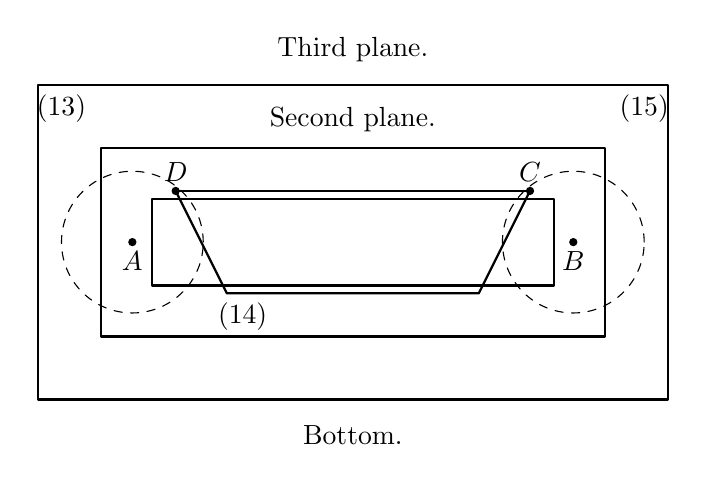
\begin{tikzpicture}[x=1cm,y=1cm,line cap=round,line join=round]
  \draw[thick] (-4,-2) rectangle (4,2);
  \draw[thick] (-3.2,-1.2) rectangle (3.2,1.2);
  \draw[thick] (-2.55,-.55) rectangle (2.55,.55);
  \node at (0,2.45) {Third plane.};
  \node at (0,1.55) {Second plane.};
  \node at (0,-2.45) {Bottom.};
  \fill (-2.8,0) circle (1.5pt) node[below] {$A$};
  \fill (2.8,0) circle (1.5pt) node[below] {$B$};
  \draw[dashed] (-2.8,0) circle (.9);
  \draw[dashed] (2.8,0) circle (.9);
  \fill (-2.25,.65) circle (1.5pt) node[above] {$D$};
  \fill (2.25,.65) circle (1.5pt) node[above] {$C$};
  \draw[thick] (-2.25,.65)--(2.25,.65);
  \draw[thick] (-2.25,.65)--(-1.6,-.65)--(1.6,-.65)--(2.25,.65);
  \node at (-3.7,1.7) {(13)};
  \node at (3.7,1.7) {(15)};
  \node at (-1.4,-.95) {(14)};
\end{tikzpicture}
\end{center}

\clearpage
\sourcepage{212}{276}
\articleno{514}
\paperhead{On the Problem of the In-and-Circumscribed Triangle.}
\journalnote{[From the Philosophical Transactions of the Royal Society of London, vol. CLXI. (for the year 1871), pp. 369--412. Received December 30, 1870,--Read February 9, 1871.]}

The problem of the In-and-Circumscribed Triangle is a particular case of that of the In-and-Circumscribed Polygon: the last-mentioned problem may be thus stated--to find a polygon such that the angles are situate in and the sides touch a given curve or curves. And we may in the first instance inquire as to the number of such polygons. In the case where the curves containing the angles and touched by the sides respectively are all of them distinct curves, the number of polygons is obtained very easily and has a simple expression: it is equal to twice the product of the orders of the curves containing the angles and of the classes of the curves touched by the sides.

For the triangle I shall need to consider also the cases in which some of the six curves are identical. I denote the angles by the small letters $a,c,e$, and the opposite sides by the capitals $B,D,F$ respectively. I use the same letters $a,c,e,B,D,F$ to denote the curves containing the angles and touched by the sides respectively; viz. the angle $a$ is situate in the curve $a$, the side $B$ touches the curve $B$, and so for the other angles and sides respectively.

\sourcepage{213}{277}
An equation such as $a=c$ or $a=B$ denotes that the curves $a,c$ or, as the case may be, the curves $a,B$ are one and the same curve: it is in general convenient to use a new letter for denoting these identical curves; viz. I write, for instance, $a=c=x$ or $a=B=x$, to denote that the curves $a,c$ or, as the case may be, the curves $a,B$ are one and the same curve $x$; the new letters thus introduced are $x,y,z$, there being in regard to them no distinction of small letters and capitals. The expression ``no identities'' denotes that the curves are all distinct. But I use also the letters $a,c,e,b,d,f,x,y,z$, and $A,C,E,B,D,F,X,Y,Z$ quantitatively, to denote the orders and classes of the curves $a,c,e,B,D,F,x,y,z$ respectively; thus, in the Table, for the case 1 ``no identities'' the number of triangles is given as $=2aceBDF$, which agrees with the before-mentioned result for the polygon: for the case 2 the several separate identities $a=c$, $a=e$, $c=e$ are of course equivalent to each other; and selecting one of them, $a=c=x$, the number of triangles is given as
\[
=2x(x-1)eBDF.
\]
There is a convenience in thus writing down the several forms $a=c$, $a=e$, $c=e$ of the identity or identities which constitute the 52 distinct cases of the Table; and I have accordingly done so throughout the Table, the expression for the number of triangles being however in each case given under one form only.

\clearpage
\sourcepage{214}{278}
\begin{landscape}
\begin{center}
\small
\begin{longtable}{c p{7.6cm} c c p{8.2cm} c}
\caption*{\textsc{Table.}}\\
\toprule
No. of Case&Specification&No. of forms&Totals&No. of triangles&Divided by\\
\midrule
\endfirsthead
\toprule
No. of Case&Specification&No. of forms&Totals&No. of triangles&Divided by\\
\midrule
\endhead
1&No identities&1&1&$2aceBDF$&\\
2&$a=c=x$;\quad $c=e$;\quad $e=a$&3&&$2x(x-1)eBDF$&\\
3&$D=F=x$;\quad $F=B$;\quad $B=D$&3&&$2X(X-1)Bace$&\\
4&$a=D=x$;\quad $c=F$;\quad $e=B$&3&&$2XaceBF$&\\
5&$a=B=x$, or $a=F$;\quad $c=D$, `` $c=B$;\quad $e=F$, `` $e=D$&6&15&$2(Xx-X-x)ceDF$&\\
6&$a=c=e=x$&1&&$\{2x(x-1)(x-2)+X\}BDF$&\\
7&$B=D=F=x$&1&&$\{2X(X-1)(X-2)+x\}ace$&\\
8&$a=c=B=x$;\quad $c=e=D$;\quad $e=a=F$&3&&$2x(x-3)(X-2)eDF$&\\
\bottomrule
\end{longtable}
\end{center}
\end{landscape}

\clearpage
\sourcepage{215}{279}
\begin{landscape}
\begin{center}
\small
\begin{longtable}{c p{8.2cm} c c p{8.2cm} c}
\caption*{\textsc{Table (continued).}}\\
\toprule
No. of Case&Specification&No. of forms&Totals&No. of triangles&Divided by\\
\midrule
\endfirsthead
\toprule
No. of Case&Specification&No. of forms&Totals&No. of triangles&Divided by\\
\midrule
\endhead
9&$D=F=e=x$;\quad $F=B=a$;\quad $B=D=c$&3&&$2X(X-3)(x-2)acB$&\\
10&$a=c=D=x$, or $a=c=F$;\quad $c=e=F$, `` $c=e=B$;\quad $e=a=B$, `` $e=a=D$&6&&$2(x-1)(Xx-X-x)eBF$&\\
11&$D=F=a=x$, or $D=F=c$;\quad $F=B=c$, `` $F=B=e$;\quad $B=D=e$, `` $B=D=a$&6&20&$2(X-1)(Xx-X-x)ceB$&\\
12&$c=e=x,\ a=D=y$;\quad $e=a,\ c=F$;\quad $a=c,\ e=B$&3&&$2x(x-1)yYBF$&\\
13&$F=B=x,\ a=D=y$;\quad $B=D,\ c=F$;\quad $D=F,\ e=B$&3&&$2X(X-1)Yyce$&\\
14&$c=e=x,\ a=B=y$, or $c=e,\ a=F$;\quad $e=a,\ c=D$, `` $e=a,\ c=B$;\quad $a=c,\ e=F$, `` $a=c,\ e=D$&6&&$2x(x-1)(Yy-Y-y)DF$&\\
15&$F=B=x,\ D=e=y$, or $F=B,\ D=c$;\quad $B=D,\ F=a$, `` $B=D,\ F=e$;\quad $D=F,\ B=c$, `` $D=F,\ B=a$&6&&(18)\quad (36)\quad $2X(X-1)(Yy-Y-y)ac$&\\
\bottomrule
\end{longtable}
\end{center}
\end{landscape}

\clearpage
\sourcepage{216}{280}
\begin{landscape}
\begin{center}
\small
\begin{longtable}{c p{8.2cm} c c p{8.2cm} c}
\caption*{\textsc{Table (continued).}}\\
\toprule
No. of Case&Specification&No. of forms&Totals&No. of triangles&Divided by\\
\midrule
\endfirsthead
\toprule
No. of Case&Specification&No. of forms&Totals&No. of triangles&Divided by\\
\midrule
\endhead
16&$c=e=x,\ D=F=y$, or $c=e,\ D=B$;\quad $e=a,\ F=B$, `` $e=a,\ F=D$;\quad $a=c,\ B=D$, `` $a=c,\ B=F$&6&&$2x(x-1)Y(Y-1)aB$&\\
17&$c=e=x,\ B=F=y$;\quad $e=a,\ D=B$;\quad $a=c,\ F=D$&3&&$2x(x-1)Y(Y-1)aD$&2\\
18&$a=D=x,\ c=B=y$, or $a=D,\ e=F$;\quad $c=F,\ e=D$, `` $c=F,\ a=B$;\quad $e=B,\ a=F$, `` $e=B,\ c=D$&6&&$2xX(Yy-Y-y)eF$&\\
19&$c=F=x,\ e=B=y$;\quad $e=B,\ a=D$;\quad $a=D,\ c=F$&3&&$2xyXYaD$&\\
20&$c=D=x,\ e=F=y$, or $c=B,\ e=D$;\quad $e=F,\ a=B$, `` $e=D,\ a=F$;\quad $a=B,\ c=D$, `` $a=F,\ c=B$&6&&$2\{xyXY-xy(X+Y)-XY(x+y)+2xy+2XY\}aB$&\\
21&$c=B=x,\ e=F=y$;\quad $e=D,\ a=B$;\quad $a=F,\ c=D$&3&45&$2\{xyXY-xy(X+Y)-XY(x+y)+2xY+2yX\}aD$&\\
22&$a=D=x,\ c=F=y,\ e=B=z$&1&&$2xyzXYZ$&\\
23&$a=B=x,\ c=D=y,\ e=F=z$;\quad $a=F,\ c=B,\ e=D$&2&&$2\{xyzXYZ-xyz(YZ+ZX+XY)-XYZ(yz+zx+xy)$\newline ${}+2xyz(X+Y+Z)+2XYZ(x+y+z)-4xyz-4XYZ\}$&\\
\bottomrule
\end{longtable}
\end{center}
\end{landscape}

\end{document}
